\documentclass[11pt]{article}

\usepackage{authblk}
\usepackage{fancyhdr}
\usepackage{float}

\usepackage[round, sort]{natbib}

\usepackage{amssymb}
\usepackage{amsmath,amsthm}

\usepackage{hyperref}
\usepackage{xcolor}
\hypersetup{
    colorlinks,
    linkcolor={red!50!black},
    citecolor={blue!50!black},
    urlcolor={blue!80!black}
}

\usepackage{multirow}
\usepackage{pgfplots}
\usepackage{arydshln}
\usepackage{paralist}
\usepackage{booktabs}
\usepackage{pbox}

\oddsidemargin 0mm
\evensidemargin 0mm
\textwidth 165mm
\textheight 205mm

\pagestyle{fancy}
\lhead{\leftmark}
\chead{}
\rhead{\rightmark}
\cfoot{\thepage}

\newcounter{rqnum} %research question number
\newcommand{\rqtherqnum}{RQ`'\therqnum}
\newcommand{\rqref}[1]{RQ\ref{#1}}

\newcounter{pnum} %pain point number
\newcommand{\ppthepnum}{P`'\thepnum}
\newcommand{\ppref}[1]{P\ref{#1}}

\newcounter{qnum} %quality number
\newcommand{\qthepnum}{Q`'\theqnum}
\newcommand{\qref}[1]{Q\ref{#1}}

\newcommand{\CC}{C\nolinebreak\hspace{-.05em}\raisebox{.4ex}{\small\bf
+}\nolinebreak\hspace{-.10em}\raisebox{.4ex}{\small\bf +}}

\pgfplotsset{compat=1.13}

\begin{document}

\title{State of the Practice for Medical Imaging Software Based on Open Source Repositories}

\author[1,*]{W.\ Spencer Smith}
\author[1]{Ao Dong}
\author[1]{Jacques Carette}
\author[2]{Michael D.\ Noseworthy}

\affil[1]{McMaster University, Computing and Software Department, {Canada}}
\affil[2]{McMaster University, Electrical \& Computer Engineering Department,
{Canada}}
\affil[*]{Corresponding Author}

\maketitle

% RQ1 to RQ4
% Some of Section 1 (Introduction)
% Sections 2 to 6 (includes looking at artifacts observed in repos)
% Some of Sections 11 to 13 (Threats to Validity, Future Work, Conclusions)

\begin{abstract}

We present the state of the practice for Medical Imaging (MI) software based on
data available in open source repositories. We selected 29 medical imaging
projects from 48 candidates and assessed 9 software qualities (installability,
correctness/ verifiability, reliability, robustness, usability, maintainability,
reusability, understandability, and visibility/transparency) by answering 108
questions for each software project. Based on the quantitative data, we ranked
the MI software with the Analytic Hierarchy Process (AHP). The top four software
products are \textit{3D Slicer}, \textit{ImageJ}, \textit{Fiji}, and
\textit{OHIF Viewer}.  Our ranking is mostly consistent with the community's
ranking, with four of our top five projects also appearing in the top five of a
list ordered by stars-per-year.  We observed 88\% of the documentation artifacts
recommended by research software development guidelines.  However, the current
state of the practice deviates from the existing guidelines because of the
rarity of some recommended artifacts (like test plans, requirements
specification, code of conduct, code style guidelines, product roadmaps, and
Application Program Interface (API) documentation).

\end{abstract}

\noindent \emph{Keywords:}
	medical imaging, research software, software engineering, software
	quality, analytic hierarchy process

\section{Introduction} \label{ch_intro}

We aim to study the state of software development practice for Medical Imaging
(MI) software using data available in open source repositories.  MI tools use
images of the interior of the body (from sources such as Magnetic Resonance
Imaging (MRI), Computed Tomography (CT), Positron Emission Tomography (PET) and
Ultrasound) to provide information for diagnostic, analytic, and medical
applications \citep{FDA2021, enwiki:1034887445, Zhang2008}.
Figure~\ref{Fig_Example}, which shows an image of the brain, highlights the
importance and value of MI. Through MI medical practitioners and researchers can
noninvasively gain insights into the human body, including information on
injuries and illnesses. Given the importance of MI software and the high number
of competing software projects, we wish to understand the merits and drawbacks
of the current development processes, tools, and methodologies. We aim to assess
through a software engineering lens the quality of the existing software with
the hope of highlighting standout examples, and providing guidelines and
recommendations for future development.

\begin{figure}[!ht]
    \begin{center}
        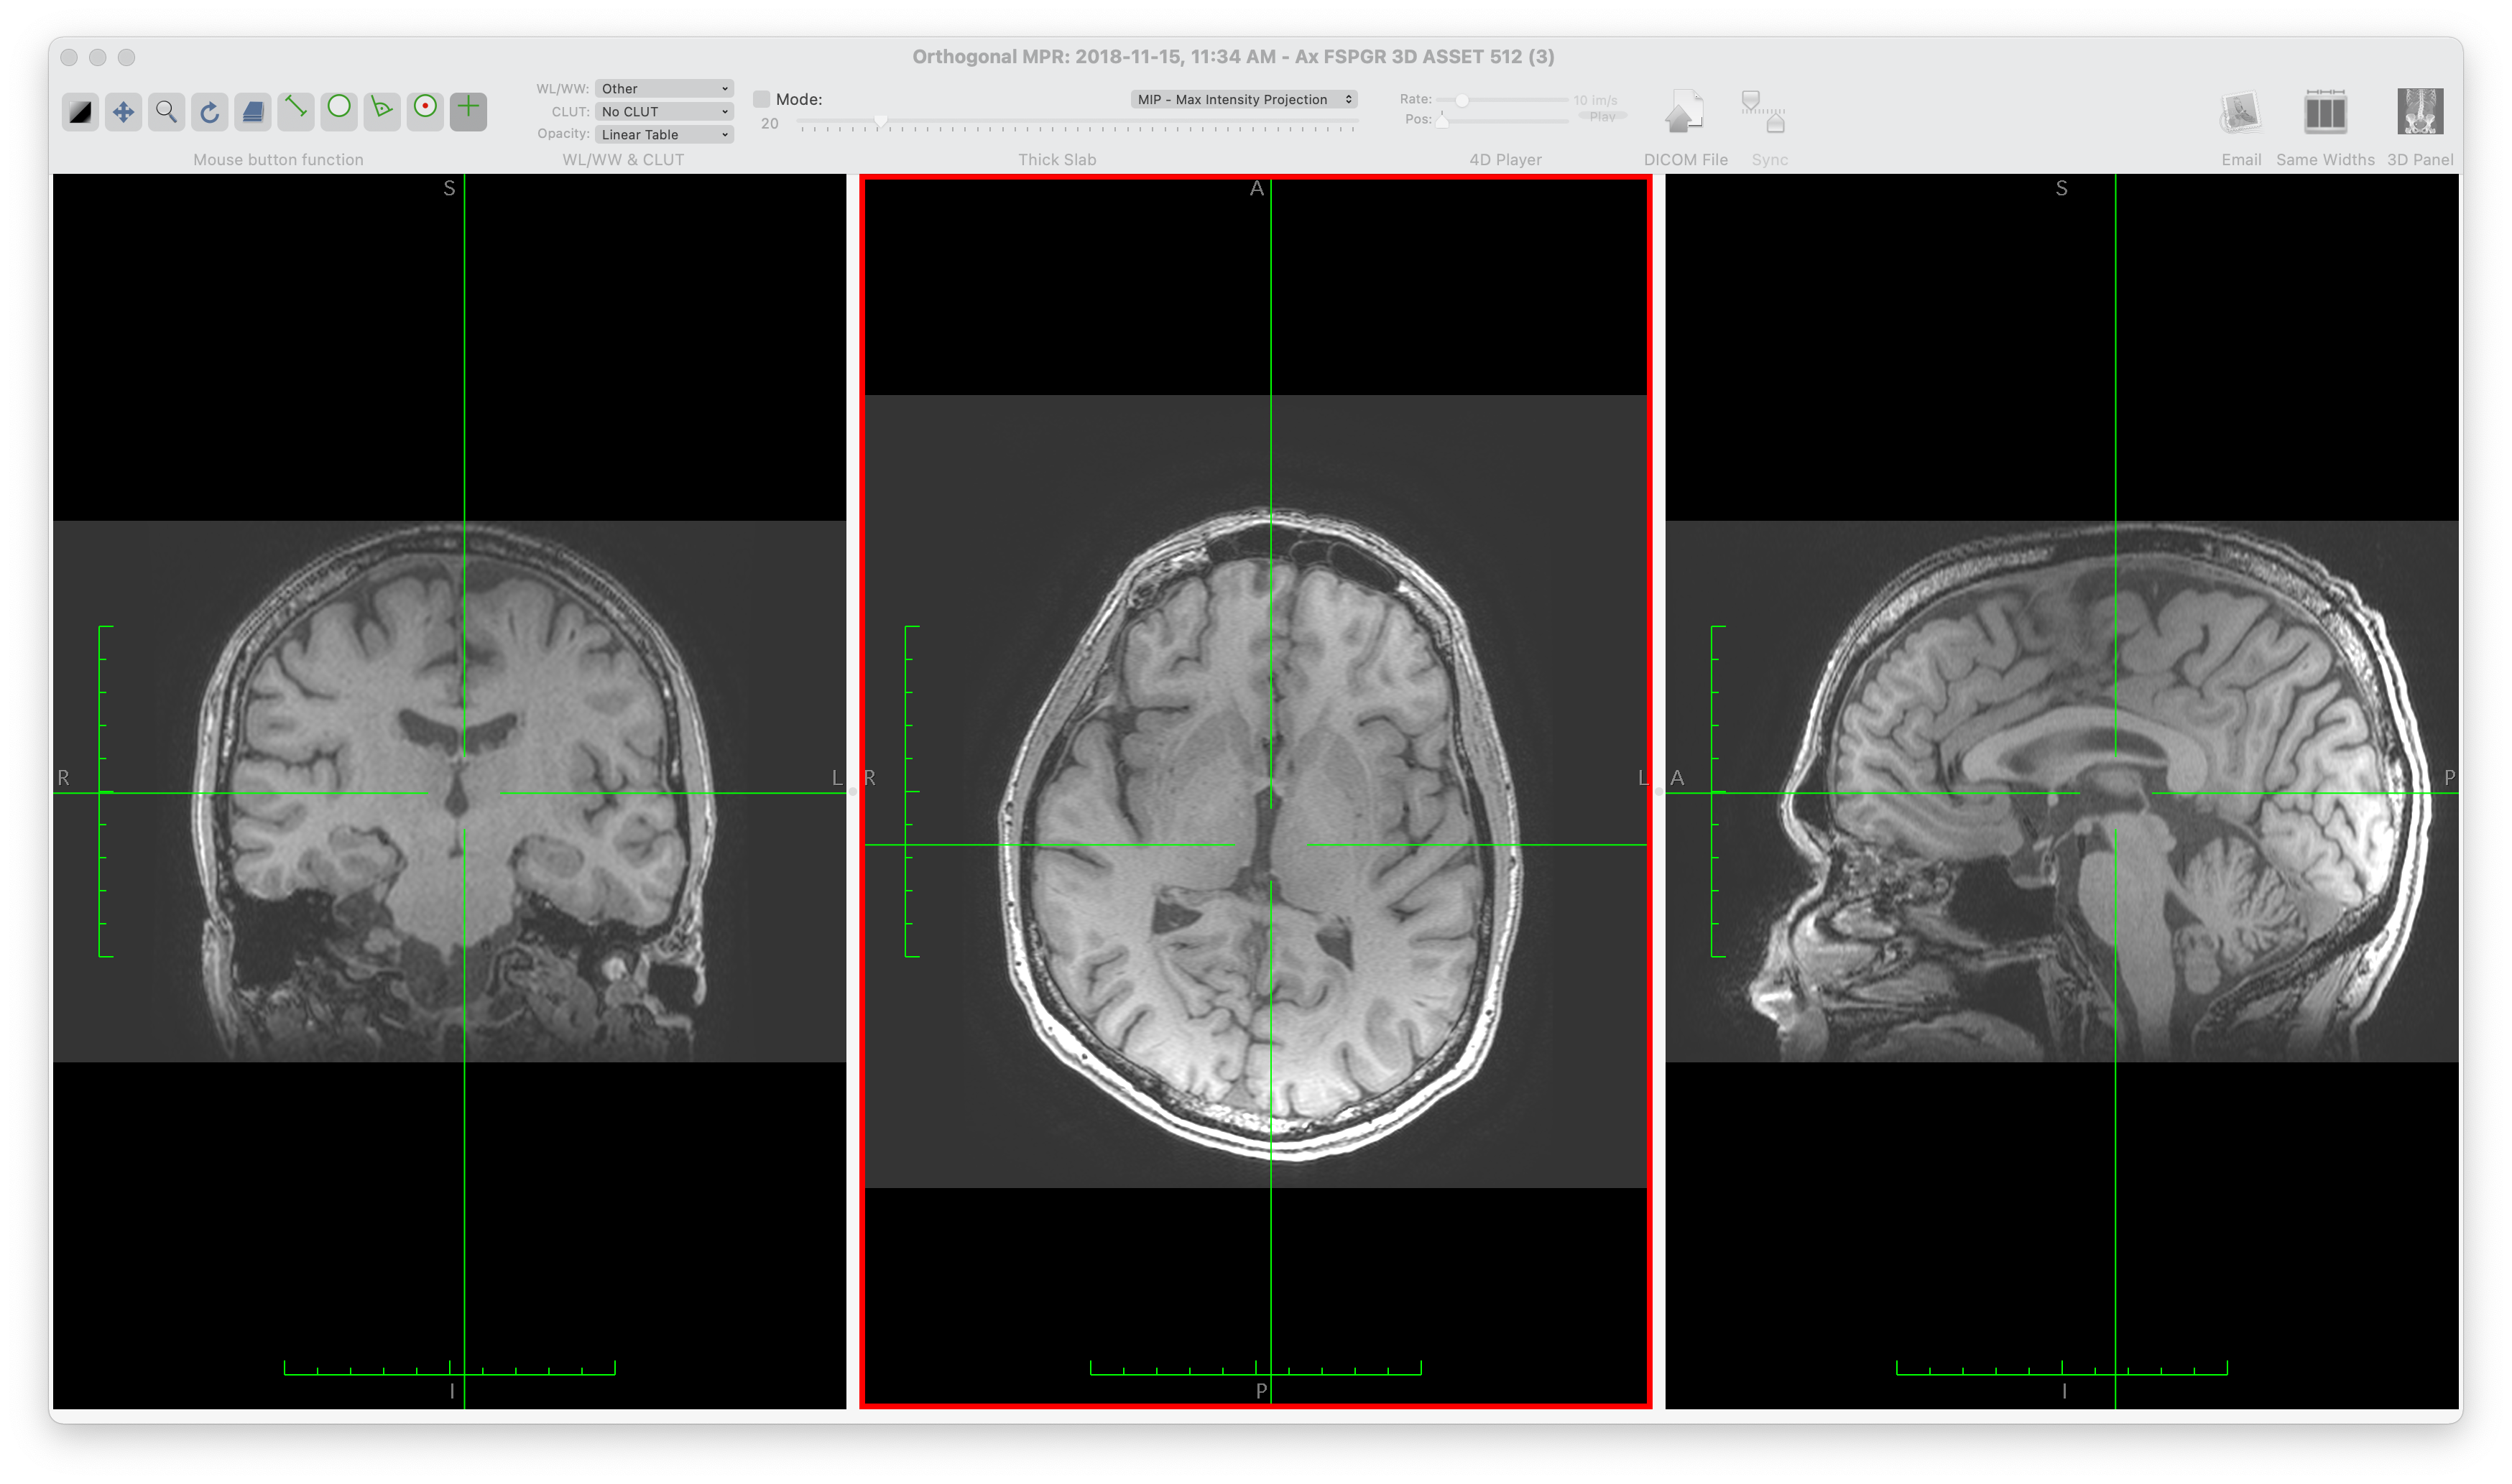
\includegraphics[scale=0.25]{MPR.png}        
    \end{center}
    \caption{Example brain image showing a multi-planar reformat using Horos
	(free open-source medical imaging/DICOM viewer for OSX, based on OsiriX)}
    \label{Fig_Example}
\end{figure}
    
\subsection{Research Questions} \label{sec_motivation}

Not only do we wish to gain insight into the state of the practice for MI
software, we also wish to understand the development of research software in
general. We wish to understand the impact of the often cited gap, or chasm,
between software engineering and research software \citep{Kelly2007,
Storer2017}. Although scientists spend a substantial proportion of their working
hours on software development \citep{Hannay2009, Prabhu2011}, many developers
learn software engineering skills by themselves or from their peers, instead of
from proper training \citep{Hannay2009}. \citet{Hannay2009} observe that many
scientists showed ignorance and indifference to standard software engineering
concepts. For instance, according to a survey by \citet{Prabhu2011}, more than
half of their 114 subjects did not use a proper debugger when coding.

To gain insight, we devised 10 research questions, which can be applied to MI,
as well as to other domains, of research software \citep{SmithEtAl2021,
SmithAndMichalski2022}.  We designed the questions to learn about the
community's interest in, and experience with, software artifacts, tools,
principles, processes, methodologies, and qualities.  When we mention artifacts
we mean the documents, scripts and code that constitutes a software development
project. Example artifacts include requirements, specifications, user manuals,
unit tests, system tests, usability tests, build scripts, API (Application
Programming Interface) documentation, READMEs, license documents, process
documents, and code.  Once we have learned what MI developers do, we then put
this information in context by contrasting MI software against the trends shown
by developers in other research software communities.

We based the structure of the paper on the research questions, so for each
research question below we point to the section that contains our answer.  We
start with identifying the relevant examples of MI software for the assessment
exercise:

\begin{enumerate}
	\item[RQ\refstepcounter{rqnum}\therqnum \label{RQ_WhatProjects}:] What MI
	software projects exist, with the constraint that the source code must be
	available for all identified projects? (Section~\ref{ch_results})
	\item [RQ\refstepcounter{rqnum}\therqnum \label{RQ_HighestQuality}:] Which
	of the projects identified in \rqref{RQ_WhatProjects} follow current best
	practices, based on evidence found by experimenting with the software and
	searching the artifacts available in each project's repository?
	(Section~\ref{ch_results})
	\item [RQ\refstepcounter{rqnum}\therqnum \label{RQ_CompareHQ2Popular}:] How
	similar is the list of top projects identified in \rqref{RQ_HighestQuality}
	to the most popular projects, as viewed by the scientific community?
	(Section~\ref{Sec_VsCommunityRanking})
    \item [RQ\refstepcounter{rqnum}\therqnum \label{RQ_CompareArtifacts}:] How
	do MI projects compare to research software in general with respect to the
	artifacts present in their repositories?
	(Section~\ref{Sec_CompareArtifacts})
\end{enumerate}

\subsection{Scope} \label{sec_scope}

To make the project feasible, we only cover MI visualization software.  As a
consequence we are excluding many other categories of MI software, including
Segmentation, Registration, Visualization, Enhancement, Quantification,
Simulation, plus MI archiving and telemedicine systems (Compression, Storage,
and Communication) (as summarized by \citet{Bankman2000} and
\citet{Angenent2006}).  We also exclude Statistical Analysis and Image-based
Physiological Modelling \citep{enwiki:1034877594} and Feature Extraction,
Classification, and Interpretation \citep{Kim2011}. Software that provides MI
support functions is also out of scope; therefore, we have not assessed the
toolkit libraries VTK \citep{SchroederEtAl2006} and ITK \citep{McCormick2014}.
Finally, Picture Archiving and Communication System (PACS), which helps users to
economically store and conveniently access images \citep{Choplin1992}, are
considered out of scope. 

\subsection{Methodology Overview}

We designed a general methodology to assess the state of the practice for
research software \citep{SmithEtAl2021, SmithAndMichalski2022}. Details can be
found in Section~\ref{ch_methods}.  Our methodology has been applied to MI
software \citep{Dong2021} and Lattice Boltzmann Solvers \citep{Michalski2021,
SmithEtAl2024}.  This methodology builds off prior work to assess the state of
the practice for such domains as Geographic Information Systems
\citep{smith2018state}, Mesh Generators \citep{smith2016state}, Seismology
software \citep{Smith2018Seismology}, and Statistical software for psychology
\citep{smith2018statistical}.  In keeping with the previous methodology, we have
maintained the constraint that the work load for measuring a given domain should
be feasible for a team as small as one person, and for a short time, ideally
around a person month of effort. We consider a person month as $20$ working days
($4$ weeks in a month, with $5$ days of work per week) at $8$ person hours per
day, or $20 \times 8 = 160$ person hours.

With our methodology, we first choose a research software domain (in the current
case MI) and identify a list of about 30 software packages. (For measuring MI we
used 29 software packages.)  We approximately measure the qualities of each
package by filling in a grading template. Compared with our previous
methodology, the new methodology also includes repository based metrics, such as
the number of files, number of lines of code, percentage of issues that are
closed, etc.  With the quantitative data in the grading template, we rank the
software with the Analytic Hierarchy Process (AHP) (Section~\ref{ch_background}
provides details).

\section{Background} \label{ch_background}

To measure the existing MI software we need the definitions of the software
qualities that we will be assessing (Section \ref{sec_software_quality}). In our
assessment we rank the software packages for each quality; therefore, this
section also provides the background on our ranking process --- the Analytic
Hierarchy Process (Section \ref{sec_AHP}).

\subsection{Software Quality Definitions} \label{sec_software_quality}

Quality is defined as a measure of the excellence or worth of an entity.  As is
common practice, we do not think of quality as a single measure, but rather as a
set of measures.  That is, quality is a collection of different qualities, often
called ``ilities.''  Below we list the 10 qualities of interest for this study.
The order of the qualities follows the order used in \citet{GhezziEtAl2003},
which puts related qualities (like correctness and reliability) together.
Moreover, the order is roughly the same as the order developers consider
qualities in practice.

\begin{itemize}
	\item \textbf{Installability} The effort required for the installation
    and/or uninstallation of software in a specified environment
    \citep{ISO/IEC25010, lenhard2013measuring}.

	\item \textbf{Correctness \& Verifiability} A program is correct if it
    matches its specification \citep[p.\ 17]{GhezziEtAl2003}.  The specification
    can either be explicitly or implicitly stated.  The related quality of
    verifiability is the ease with which the software components or the
    integrated product can be checked to demonstrate its correctness. 

	\item \textbf{Reliability} The probability of failure-free operation of a
	computer program in a specified environment for a specified time
	\citep{musa1987software}, \citep[p.\ 357]{GhezziEtAl2003}.

	\item \textbf{Robustness} Software possesses the characteristic of
	robustness if it behaves ``reasonably'' in two situations: i) when it
	encounters circumstances not anticipated in the requirements specification,
	and ii) when users violate the assumptions in its requirements specification 
	\citep[p.\ 19]{GhezziEtAl2003}, \citep{boehm2007software}.

	\item \textbf{Usability} ``The extent to which a product can be used by
	specified users to achieve specified goals with effectiveness, efficiency,
	and satisfaction in a specified context of use'' \citep{ISO/TR16982:2002,
	ISO9241-11:2018}.

	\item \textbf{Maintainability} The effort with which a software system or
	component can be modified to i) correct faults; ii) improve performance or
	other attributes; iii) satisfy new requirements
	\citep{IEEEStdGlossarySET1990, boehm2007software}.

	\item \textbf{Reusability} ``The extent to which a software component can be
	used with or without adaptation in a problem solution other than the one for
	which it was originally developed'' \citep{kalagiakos2003non}.

	\item \textbf{Understandability} ``The capability of the software product to
	enable the user to understand whether the software is suitable, and how it
	can be used for particular tasks and conditions of use'' \citep{iso2001iec}.

	\item \textbf{Visibility/Transparency} The extent to which all the steps
	of a software development process and the current status of it are conveyed
	clearly \citep[p.\ 32]{GhezziEtAl2003}.

\end{itemize}

\subsection{Analytic Hierarchy Process (AHP)} \label{sec_AHP}

Saaty developed AHP in the 1970s, and people have widely used it since to make
and analyze multiple criteria decisions \citep{VaidyaEtAl2006}. AHP organizes
multiple criteria in a hierarchical structure and uses pairwise comparisons
between alternatives to calculate relative ratios \citep{Saaty1990}. AHP works
with sets of $n$ \textit{options} and $m$ \textit{criteria}.  In our project
$n=29$ and $m=9$ since there are 29 options (software products) and 9 criteria
(qualities). We rank the software for each of the qualities, and then we combine
the quality rankings into an overall ranking based on the relative priorities
between qualities.

The first step for ranking the software choices for a given quality involves a
pairwise comparison between each of the $n$ software options for that quality.
AHP expresses the comparison through an $n \times n$ matrix $A$. When comparing
option $i$ and option $j$, the value of $A_{ij}$ is decided as follows, with the
value of $A_{ji}$ generally equal to $1/A_{ij}$ \citep{Saaty1990}: $A_{ij} = 1$
if criterion $i$ and criterion $j$ are equally important, while $A_{ij} = 9$ if
criterion $i$ is extremely more important than criterion $j$.  The natural
numbers between 1 and 9 are used to show the different levels of relative
importance between these two extremes. The above assumes that option $i$ is of
equal, or more, importance compared to option $j$ ($i \geq j$).  If that is not
the case, we reverse $i$ and $j$ and determine $A_{ji}$ first, then $A_{ij} =
1/A_{ji}$.

Section~\ref{sec_grading_software} shows how we measure the software via a
grading template.  For the AHP process, the relevant measure is the subjective
score from $1$ to $10$ for each quality for each package. To turn these
subjective measures $x_{\text{sub}}$ and $y_{\text{sub}}$ into Saaty's
pair-wise scores for option $x$ versus option $y$, respectively, we use the
following calculation:
\[
\begin{cases}
\min\{9, x_{\text{sub}} - y_{\text{sub}} + 1\} & x_{\text{sub}} \geq y_{\text{sub}} \\
1 / \min\{9, y_{\text{sub}} - x_{\text{sub}} + 1\} & x_{\text{sub}} < y_{\text{sub}}
\end{cases}
\]

\noindent For example, we measured the usability for 3D Slicer and Ginkgo CADx
as $8$ and $7$, respectively; therefore, on the 9-point scale, 3D Slicer compared
to Ginkgo CADx is 2 and Ginkgo CADx versus 3D Slicer is 1/2, as shown in the
sample AHP calculations (Table~\ref{Tbl_SampleAHP}).

The second step is to calculate the priority vector $w$ from $A$.  The
vector $w$ ranks the software options by how well they achieve the given
quality.  The priority vector can be calculated by solving the equation
\citep{Saaty1990}:
\begin{equation} 
    A w = \lambda_{\text{max}} w,
\end{equation}
where $\lambda_{\text{max}}$ is the maximal eigenvalue of $A$.  In this project,
$w$ is approximated with the classic \textit{mean of normalized values} approach
\citep{AlessioEtAl2006}:

\begin{equation}
w_i = \frac{1}{n}\sum_{j=1}^{n}\frac{A_{ij}}{\sum_{k=1}^{n}A_{kj}}
\end{equation}

Table~\ref{Tbl_SampleAHP} summarizes the above two steps for the quality of
installability.  The matrix $A$ is shown in the first set of columns, then the
normalized version of $A$ and finally the average of the normalized values to
form the vector $w$ in the last column.

\begin{table}[h!]
\begin{center}
\begin{tabular}{ l c c c c c | c c c c c | c }
 \toprule
 ~ & \multicolumn{5}{c|}{$A_{ij}$} & \multicolumn{5}{c|}{${A_{ij}}/{\sum_{k=1}^{n}A_{kj}}$} & ~\\
 \midrule
 ~ & \rotatebox{90}{3D Slicer} & \rotatebox{90}{Ginkgo} & \rotatebox{90}{XMedCon} & $\cdots$ & \rotatebox{90}{Gwyddion} & \rotatebox{90}{3D Slicer} & \rotatebox{90}{Ginkgo} & \rotatebox{90}{XMedCon} & $\cdots$ & \rotatebox{90}{Gwyddion} & AVG \\
 \midrule
 3D Slicer & 1 & 2 & 4 & $\cdots$ & 2 & 0.071 & 0.078 & 0.060 & $\cdots$ & 0.078 & 0.068\\
 Ginkgo & 1/2 & 1 & 3 & $\cdots$ & 1 & 0.036 & 0.039 & 0.045 & $\cdots$ & 0.039 & 0.041\\
 XMedCon & 1/4 & 1/3 & 1 & $\cdots$ & 1/3 & 0.018 & 0.013 & 0.015 & $\cdots$ & 0.013 & 0.015\\
 $\vdots$ & $\vdots$ & $\vdots$ & $\vdots$ & $\ddots$ & $\vdots$ & $\vdots$ & $\vdots$ & $\vdots$ & $\ddots$ & $\vdots$ & $\vdots$\\
 Gwyddion & 1/2 & 1 & 3 & $\cdots$ & 1 & 0.036 & 0.039 & 0.045 & $\cdots$ & 0.039 & 0.041\\  
 \midrule
 SUM = & 14.01 & 25.58 & 66.75 & $\cdots$ & 25.58 & 1.000 & 1.000 & 1.000 & $\cdots$ & 1.000 & 1.000\\
 \bottomrule
\end{tabular}
\end{center}
\caption{Sample AHP Calculations for the Quality of Usability} \label{Tbl_SampleAHP}
\end{table}

We repeat the first and second steps for each of the qualities.  The third step
combines the quality rankings into an overall ranking.  Following AHP, we need
to first prioritize the qualities.  The AHP method finds the priority of quality
$i$ ($p_i$) in the same way that the score ($w_j$) was found for software
package $j$ evaluated for a given quality (as shown above).  That is, we
conduct a pairwise comparison between the priority of different qualities to
construct the $m \times m$ matrix $A$, and then we take the mean of normalized
values for row $i$ to find the priority value $p_i$ for quality $i$.  If we
introduce the notation that $w^i_j$ is the score for quality $i$ for package
$j$, then the overall score $S_j$ for package $j$ is found via:

$$S_j = \sum_{i=1}^m w^i_j p_i$$ 

\section{Methodology} \label{ch_methods}

We developed a methodology for evaluating the state of the practice of research
software \citep{SmithEtAl2021, SmithAndMichalski2022}.  The methodology can be
instantiated for a specific domain of scientific software, which in the current
case is medical imaging software for visualization.  Our methodology involves
and engages a domain expert partner throughout, as discussed in
Section~\ref{sec_vet_software_list}.  The three main steps of the methodology
are:

\begin{enumerate}
\item Identify list of representative software packages
(Section~\ref{sec_software_selection});
\item Measure (or grade) the selected software
(Section~\ref{sec_grading_software});
\item Answer the research questions (as given in Section~\ref{sec_motivation}).
\end{enumerate}

In the sections below we provide additional detail on the above steps, while
concurrently giving examples of how we applied the methodology to the MI domain.

\subsection{Interaction With Domain Expert} \label{sec_vet_software_list}

The Domain Expert is an important member of the state of the practice assessment
team. Pitfalls exist if non-experts attempt to acquire an authoritative list of
software, or try to definitively rank the software. Non-experts have the problem
that they can only rely on information available on-line, which has the
following drawbacks:
\begin{inparaenum}[i)]
  \item the on-line resources could have false or inaccurate information; and,
  \item the on-line resources could leave out relevant information that is so
in-grained with experts that nobody thinks to explicitly record it.
\end{inparaenum}

Domain experts may be recruited from academia or industry.  The only
requirements are knowledge of the domain and a willingness to be engaged in the
assessment process.  The Domain Expert does not have to be a software developer,
but they should be a user of domain software.  Given that the domain experts are
likely to be busy people, the measurement process cannot put too much of a burden
on their time.  For the current assessment, our Domain Expert (and paper
co-author) is Dr.\ Michael Noseworthy, Professor of Electrical and Computer
Engineering at McMaster University, Co-Director of the McMaster School of
Biomedical Engineering, and Director of Medical Imaging Physics and Engineering
at St.\ Joseph's Healthcare, Hamilton, Ontario, Canada.  

In advance of the first meeting with the Domain Expert, they are asked to
create a list of top software packages in the domain.  This is done to help
the expert get in the right mind set in advance of the meeting.  Moreover,
by doing the exercise in advance, we avoid the potential pitfall of the expert
approving the discovered list of software without giving it adequate thought.

The Domain Experts are asked to vet the collected data and analysis.  In
particular, they are asked to vet the proposed list of software packages and the
AHP ranking.  These interactions can be done either electronically or with
in-person (or virtual) meetings.

\subsection{List of Representative Software} \label{sec_software_selection}

We have a two-step process for selecting software packages: i) identify software
candidates in the chosen domain; and, ii) filter the list to remove less
relevant members \citep{SmithEtAl2021}.

We initially identified 48 MI candidate software projects from the literature
\citep{Bjorn2017, Bruhschwein2019, Haak2015}, on-line articles \citep{Emms2019,
Hasan2020, Mu2019}, and forum discussions \citep{Samala2014}.  The full list of
48 packages is available in \citet{Dong2021}.  To reduce the length of the list
to a manageable number (29 in this case, as given in Section~\ref{ch_results}),
we filtered the original list as follows:

\begin{enumerate}

\item We removed the packages that did not have source code available, such as
\textit{MicroDicom}, \textit{Aliza}, and \textit{jivex}.

\item We focused on the MI software that provides visualization functions, as
described in Section~\ref{sec_scope}. Furthermore, we removed seven packages that were
toolkits or libraries, such as \textit{VTK}, \textit{ITK}, and \textit{dcm4che}.
We removed another three that were for PACS.

\item We removed \textit{Open Dicom Viewer}, since it has not received any
updates in a long time (since 2011).

\end{enumerate}

The Domain Expert provided a list of his top 12 software packages.  We compared
his list to our list of 29.  We found 6 packages were on both lists: \textit{3D
Slicer}, \textit{Horos}, \textit{ImageJ}, \textit{Fiji}, \textit{MRIcron} (we
actually use the update version \textit{MRIcroGL}) and \textit{Mango} (we
actually use the web version \textit{Papaya}).  Six software packages
(\textit{AFNI}, \textit{FSL}, \textit{Freesurfer}, \textit{Tarquin},
\textit{Diffusion Toolkit}, and \textit{MRItrix}) were on the Domain Expert
list, but not on our filtered list.  However, when we examined those packages,
we found they were out of scope, since their primary function was not
visualization.  The Domain Expert agreed with our final choice of 29 packages.

\subsection{Grading Software} \label{sec_grading_software}

We grade the selected software using the measurement template summarized in
\citet{SmithEtAl2021}.  The template provides measures of the qualities listed
in Section~\ref{sec_software_quality}.
For each software package, we fill in the template questions. To stay within the
target of 160 person hours to measure the domain, we allocated between one and
four hours for each package. Project developers can be contacted for help
regarding installation, if necessary, but we impose a cap of about two hours on
the installation process, to keep the overall measurement time feasible.
Figure~\ref{fg_grading_template_example} shows an excerpt of the spreadsheet.
The spreadsheet includes a column for each measured software package. 

\begin{figure}[!ht]
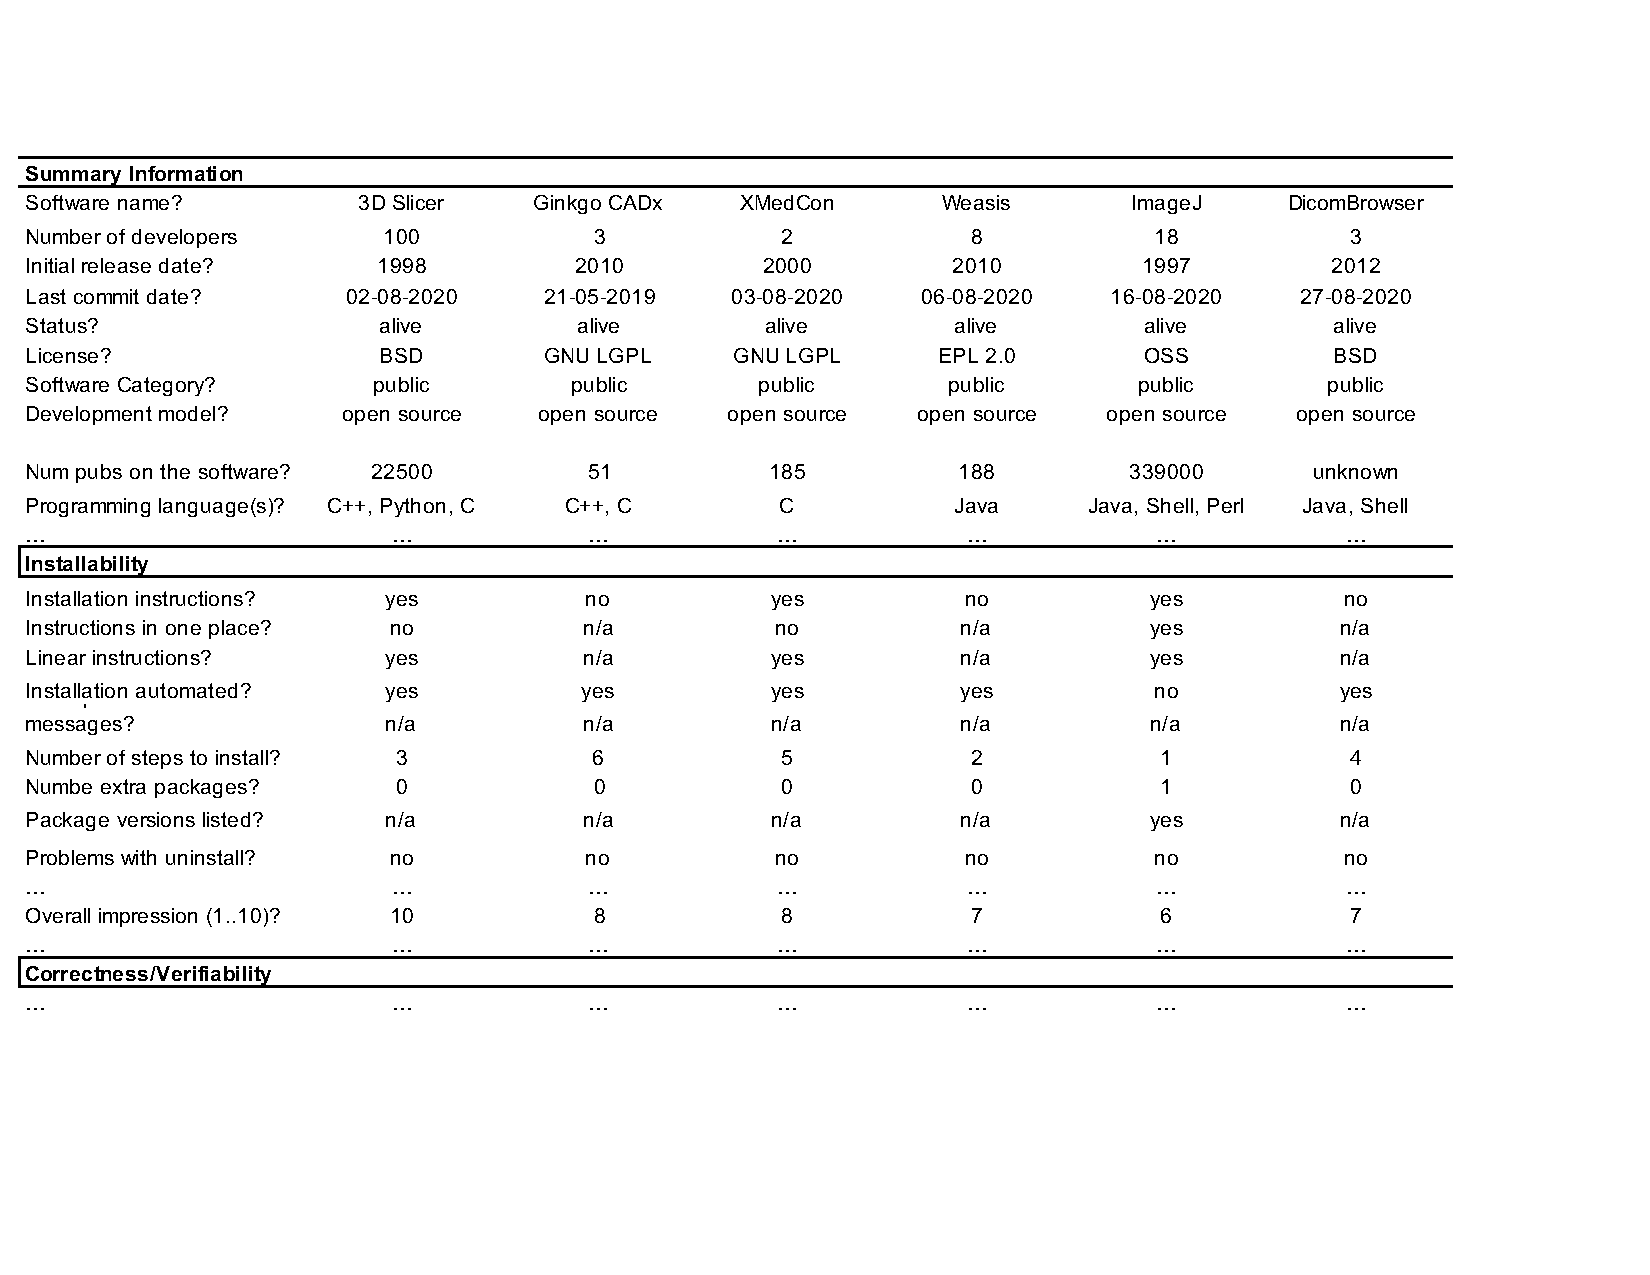
\includegraphics[scale=0.66]{template.pdf}
\caption{Grading template example}
\label{fg_grading_template_example}
\end{figure}

The full template consists of 108 questions categorized under 9 qualities.  We
designed the questions to be unambiguous, quantifiable, and measurable with
limited time and domain knowledge. We group the measures under headings for each
quality, and one for summary information. The summary information (shown in
Figure~\ref{fg_grading_template_example}) is the first section of the template.
This section summarizes general information, such as the software name, purpose,
platform, programming language, publications about the software, the first
release and the most recent change date, website, source code repository of the
product, number of developers, etc.  We follow the definitions given by
\citet{GewaltigAndCannon2012} for the software categories.  Public means
software intended for public use.  Private means software aimed only at a
specific group, while the concept category is for software written simply to
demonstrate algorithms or concepts. The three categories of development models
are (open source, free-ware and commercial) are discussed in
Section~\ref{sec_software_categories}.  Information in the summary section sets
the context for the project, but it does not directly affect the grading scores.

For measuring each quality, we ask several questions and the typical answers are
among the collection of ``yes'', ``no'', ``n/a'', ``unclear'', a number, a
string, a date, a set of strings, etc. The grader assigns each quality an
overall score, between 1 and 10, based on all the previous questions.  Several
of the qualities use the word ``surface''.  This is to highlight that, for these
qualities in particular, the best that we can do is a shallow measure.  For
instance, we are not currently doing any experiments to measure usability.
Instead, we are looking for an indication that the developers considered
usability.  We do this by looking for cues in the documentation, like a getting
started manual, a user manual and a statement of expected user characteristics.
Below is a summary of how we assess adoption of best practices by measuring each
quality.

\begin{itemize}

\item \textbf{Installability} We assess the following: 
\begin{inparaenum}[i)]
    \item existence and quality of installation instructions;
    \item the quality of the user experience via the ease of following
    instructions, number of steps, automation tools; and,
    \item whether there is a means to verify the installation.
\end{inparaenum}
If any problem interrupts the process of installation or uninstallation, we give
a lower score. We also record the Operating System (OS) used for the
installation test.

% move the definitions here; it seems repetitive the way it is now - maybe
% remove the definitions?
\item \textbf{Correctness \& Verifiability} We check each project to identify
any techniques used to ensure this quality, such as literate programming,
automated testing, symbolic execution, model checking, unit tests, etc. We also
examine whether the projects use Continuous Integration and Continuous Delivery
(CI/CD). For verifiability, we go through the documents of the projects to check
for the presence of requirements specifications, theory manuals, and getting
started tutorials. If a getting started tutorial exists and provides expected
results, we follow it to check the correctness of the output.

\item \textbf{Surface Reliability} We check the following: 
\begin{inparaenum}[i)]
    \item whether the software breaks during installation;
    \item the operation of the software following the getting started tutorial
    (if present);
    \item whether the error messages are descriptive; and,
    \item whether we can recover the process after an error.
\end{inparaenum}

\item \textbf{Surface Robustness} We check how the software handles
unexpected/unanticipated input. For example, we prepare broken image files for
MI software packages that load image files. We use a text file (.txt) with a
modified extension name (.dcm) as an unexpected/unanticipated input. We load a
few correct input files to ensure the function is working correctly before
testing the unexpected/unanticipated ones.

\item \textbf{Surface Usability} We examine the project's documentation,
checking for the presence of getting started tutorials and/or a user manual. We
also check whether users have channels to request support, such as an e-mail
address, or issue tracker. Our impressions of usability are based on our
interaction with the software during testing.  In general, an easy-to-use
graphical user interface will score high.

\item \textbf{Maintainability} We believe that the artifacts of a project,
including source code, documents, and building scripts, significantly influence
its maintainability. Thus, we check each project for the presence of such
artifacts as API documentation, bug tracker information, release notes, test
cases, and build scripts. We also check for the use of tools supporting issue
tracking and version control, the percentages of closed issues, and the
proportion of comment lines in the code.

\item \textbf{Reusability} We count the total number of code files for each
project. Projects with numerous components potentially provide more choices for
reuse. Furthermore, well-modularized code, which tends to have smaller parts in
separate files, is typically easier to reuse. Thus, we assume that projects with
more code files and fewer Lines of Code (LOC) per file are more reusable. We also
consider projects with API documentation as delivering better reusability.

\item \textbf{Surface Understandability} Given that time is a constraint, we
cannot look at all code files for each project; therefore, we randomly examine
10 code files for their understandability. We check the code's style within each
file, such as whether the identifiers, parameters, indentation, and formatting
are consistent, whether the constants (other than 0 and 1) are not hardcoded, and
whether the code is modularized. We also check the descriptive information for
the code, such as documents mentioning the coding standard, the comments in the
code, and the descriptions or links for details on algorithms in the code. 

\item \textbf{Visibility/Transparency} To measure this quality, we check the
existing documents to find whether the software development process and
current status of a project are visible and transparent. We examine the
development process, current status, development environment, and release notes
for each project.
\end{itemize}

As part of filling in the measurement template, we use freeware tools to collect
repository related data. \href{https://github.com/tomgi/git_stats}{GitStats}
\citep{Gieniusz2019} is used to measure the number of binary files as well as
the number of added and deleted lines in a repository. We also use this tool to
measure the number of commits over different intervals of time.
\href{https://github.com/boyter/scc}{Sloc Cloc and Code (scc)}
\citep{Boyter2021} is used to measure the number of text based files as well as
the number of total, code, comment, and blank lines in a repository.

Both tools measure the number of text-based files in a git repository and lines
of text in these files. Based on our experience, most text-based files in a
repository contain programming source code, and developers use them to compile
and build software products. A minority of these files are instructions and
other documents. So we roughly regard the lines of text in text-based files as
lines of programming code. The two tools usually generate similar but not
identical results. From our understanding, this minor difference is due to the
different techniques to detect if a file is text-based or binary.

For projects on GitHub we manually collect additional information, such as the
numbers of stars, forks, people watching this repository, open pull requests,
closed pull requests, and the number of months a repository has been on GitHub.
We need to take care with the project creation date, since a repository can have
a creation date much earlier than the first day on GitHub.  For example, the
developers created the git repository for \textit{3D Slicer} in 2002, but did
not upload a copy of it to GitHub until 2020. Some GitHub data can be found
using its GitHub Application Program Interface (API) via the following url:
\textit{https://api.github.com/repos/[owner]/[repository]} where [owner] and
[repository] are replaced by the repo specific values. The number of months a
repository has been on GitHub helps us understand the average change of metrics
over time, like the average new stars per month. 

The repository measures help us in many ways. Firstly, they help us get a fast
and accurate project overview. For example, the number of commits over the last
12 months shows how active a project has been, and the number of stars and forks
may reveal its popularity (used to assess \rqref{RQ_CompareHQ2Popular}).
Secondly, the results may affect our decisions regarding the grading scores for
some software qualities. For example, if the percentage of comment lines is low,
we double-check the understandability of the code; if the ratio of open versus
closed pull requests is high, we pay more attention to maintainability.

As in \citet{SmithEtAl2016}, Virtual machines (VMs) were used to provide an
optimal testing environment for each package. We used VMs because it is easier
to start with a fresh environment, without having to worry about existing
libraries and conflicts. Moreover, when the tests are complete the VM can be
deleted, without any impact on the host operating system. The most significant
advantage of using VMs is to level the playing field. Every software install
starts from a clean slate, which removes ``works-on-my-computer'' errors. When
filling in the measurement template, the grader notes the details for each VM,
including hypervisor and operating system version.

When grading the software, we found 27 out of the 29 packages are compatible
with two or three different OSes, such as Windows, macOS, and Linux, and 5 of
them are browser-based, making them platform-independent. However, in the
interest of time, we only performed the measurements for each project by
installing it on one of the platforms.  When it was an option, we selected
Windows as the host OS.

\section{Measurement Results} \label{ch_results}

Table~\ref{tab_final_list} shows the 29 software packages that we measured,
along with summary data collected in the year 2020. We arrange the items in
descending order of LOC. We found the initial release dates (Rlsd) for most
projects and marked the two unknown dates with ``?''. The date of the last
update is the date of the latest update, at the time of measurement. We found
funding information (Fnd) for only eight projects.  For the Number Of
Contributors (NOC) we considered anyone who made at least one accepted commit as
a contributor. The NOC is not usually the same as the number of long-term
project members, since many projects received change requests and code from the
community.  With respect to the OS, 25 packages work on all three OSs: Windows
(W), macOS (M), and Linux (L). Although the usual approach to cross-platform
compatibility was to work natively on multiple OSes, five projects achieved
platform-independence via web applications. The full measurement data for all
packages is available in \citet{Dong2021-Data}.

\begin{table}[!ht]
\centering
\begin{tabular}{p{6cm}lllllllll}
\toprule
\multirow{2}{*}{Software} & \multirow{2}{*}{Rlsd} & \multirow{2}{*}{Updated} & \multirow{2}{*}{Fnd} & \multirow{2}{*}{NOC} & \multirow{2}{*}{LOC} & \multicolumn{3}{c}{OS} & \multirow{2}{*}{Web} \\ \cline{7-9}
 &  &  &  &  &  & W & M & L &  \\ \midrule
ParaView \citep{Ahrens2005} & 2002 & 2020-10 & \checkmark & 100 & 886326 & \checkmark & \checkmark & \checkmark & \checkmark \\
Gwyddion \citep{Nevcas2012} & 2004 & 2020-11 &  & 38 & 643427 & \checkmark & \checkmark & \checkmark &  \\
Horos \citep{horosproject2020} & ? & 2020-04 &  & 21 & 561617 &  & \checkmark &  &  \\
OsiriX Lite \citep{PixmeoSARL2019} & 2004 & 2019-11 &  & 9 & 544304 &  & \checkmark &  &  \\
3D Slicer \citep{Kikinis2014} & 1998 & 2020-08 & \checkmark & 100 & 501451 & \checkmark & \checkmark & \checkmark &  \\
Drishti \citep{Limaye2012} & 2012 & 2020-08 &  & 1 & 268168 & \checkmark & \checkmark & \checkmark &  \\
Ginkgo CADx \citep{Wollny2020} & 2010 & 2019-05 &  & 3 & 257144 & \checkmark & \checkmark & \checkmark &  \\
GATE \citep{Jan2004} & 2011 & 2020-10 &  & 45 & 207122 &  & \checkmark & \checkmark &  \\
3DimViewer \citep{TESCAN2020} & ? & 2020-03 & \checkmark & 3 & 178065 & \checkmark & \checkmark &  &  \\
medInria \citep{Fillard2012} & 2009 & 2020-11 &  & 21 & 148924 & \checkmark & \checkmark & \checkmark &  \\
BioImage Suite Web \citep{Papademetris2005} & 2018 & 2020-10 & \checkmark & 13 & 139699 &
\checkmark & \checkmark & \checkmark & \checkmark \\
Weasis \citep{Roduit2021} & 2010 & 2020-08 &  & 8 & 123272 & \checkmark & \checkmark & \checkmark &  \\
AMIDE \citep{Loening2017} & 2006 & 2017-01 &  & 4 & 102827 & \checkmark & \checkmark & \checkmark &  \\
XMedCon \citep{Nolf2003} & 2000 & 2020-08 &  & 2 & 96767 & \checkmark & \checkmark & \checkmark &  \\
ITK-SNAP \citep{Yushkevich2006} & 2006 & 2020-06 & \checkmark & 13 & 88530 & \checkmark & \checkmark & \checkmark &  \\
Papaya \citep{UTHSCSA2019} & 2012 & 2019-05 &  & 9 & 71831 & \checkmark & \checkmark & \checkmark &  \\
OHIF Viewer \citep{Ziegler2020} & 2015 & 2020-10 &  & 76 & 63951 & \checkmark & \checkmark & \checkmark & \checkmark \\
SMILI \citep{Chandra2018} & 2014 & 2020-06 &  & 9 & 62626 & \checkmark & \checkmark & \checkmark &  \\
INVESALIUS 3 \citep{Amorim2015} & 2009 & 2020-09 &  & 10 & 48605 & \checkmark & \checkmark & \checkmark &  \\
dwv \citep{Martelli2021} & 2012 & 2020-09 &  & 22 & 47815 & \checkmark & \checkmark & \checkmark & \checkmark \\
DICOM Viewer \citep{Afsar2021} & 2018 & 2020-04 & \checkmark & 5 & 30761 & \checkmark & \checkmark & \checkmark &  \\
MicroView \citep{ParallaxInnovations2020} & 2015 & 2020-08 &  & 2 & 27470 & \checkmark & \checkmark & \checkmark &  \\
MatrixUser \citep{Liu2016} & 2013 & 2018-07 &  & 1 & 23121 & \checkmark & \checkmark & \checkmark &  \\
Slice:Drop \citep{Haehn2013} & 2012 & 2020-04 &  & 3 & 19020 & \checkmark & \checkmark & \checkmark & \checkmark \\
dicompyler \citep{Panchal2010} & 2009 & 2020-01 &  & 2 & 15941 & \checkmark & \checkmark &  &  \\
Fiji \citep{Schindelin2012} & 2011 & 2020-08 & \checkmark & 55 & 10833 & \checkmark & \checkmark & \checkmark &  \\
ImageJ \citep{Rueden2017} & 1997 & 2020-08 & \checkmark & 18 & 9681 & \checkmark & \checkmark & \checkmark &  \\
MRIcroGL \citep{Rorden2021} & 2015 & 2020-08 &  & 2 & 8493 & \checkmark & \checkmark & \checkmark &  \\
DicomBrowser \citep{Archie2012} & 2012 & 2020-08 &  & 3 & 5505 & \checkmark & \checkmark & \checkmark &  \\ \bottomrule
\end{tabular}
\caption{Final software list (sorted in descending order of the number of Lines
Of Code (LOC))}
\label{tab_final_list}
\end{table}

Figure \ref{fig_language} shows the primary languages versus the number of
projects using them.  The primary language is the language used for the majority
of the project's code; in most cases projects also use other languages.  The
most popular language is \CC, with almost 40\% of projects (11 of 29).  The two
least popular choices are Pascal and Matlab, with around 3\% of projects each
(1 of 29).

\begin{figure}[!ht]
\centering
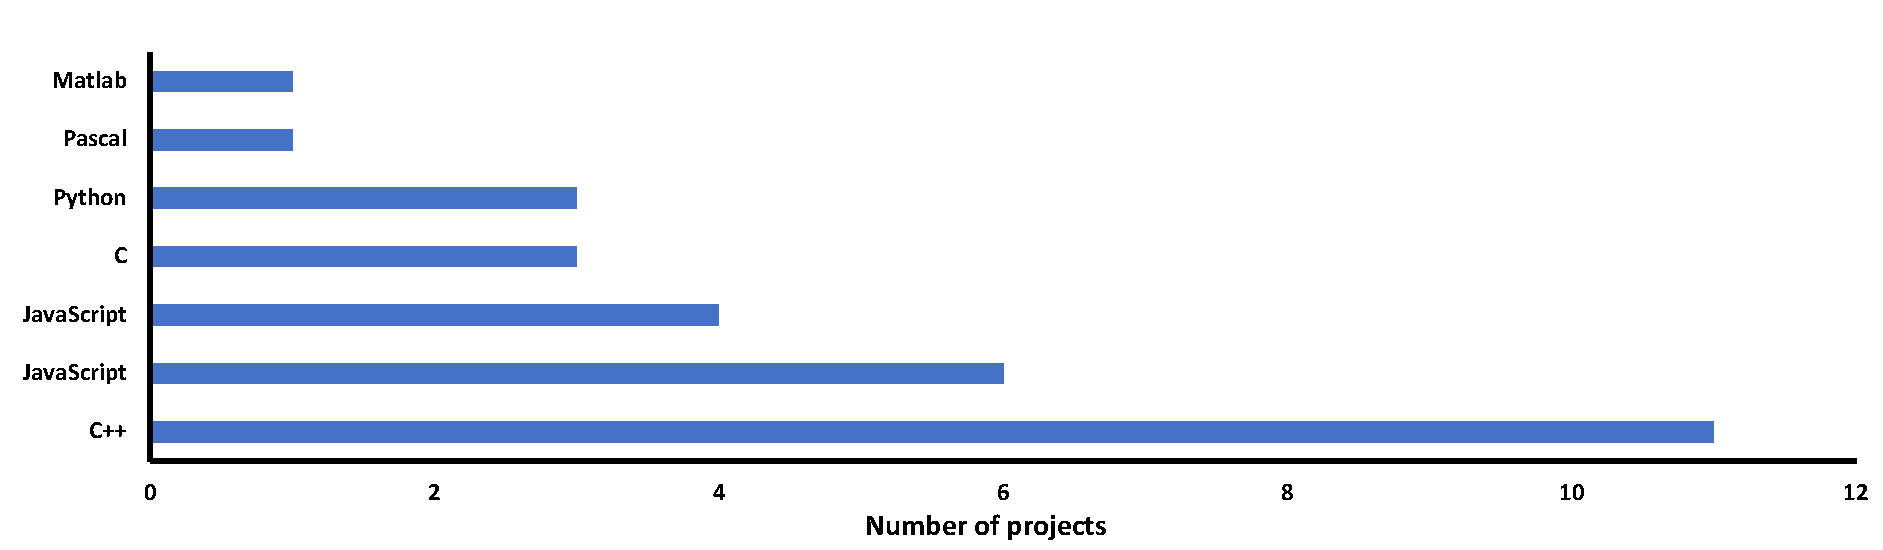
\includegraphics[scale=0.5]{PrimaryLanguages.pdf}
\centering
\caption{\label{fig_language}Primary languages versus number of projects}
\end{figure}

\subsection{Installability} \label{sec_result_installability}

Figure \ref{fg_installability_scores} lists the installability scores.  We found
installation instructions for 16 projects. Among the ones without instructions,
\textit{BioImage Suite Web} and \textit{Slice:Drop} do not need installation,
since they are web applications. Installing 10 of the projects required extra
dependencies. Five of them are web applications (as shown in
Table~\ref{tab_final_list}) and depend on a browser; \textit{dwv}, \textit{OHIF
Viewer}, and \textit{GATE} needs extra dependencies to build; \textit{ImageJ}
and	\textit{Fiji} need an unzip tool; \textit{MatrixUser} is based on Matlab;
\textit{DICOM Viewer} needs to work on a Nextcloud platform.

\begin{figure}[!ht]
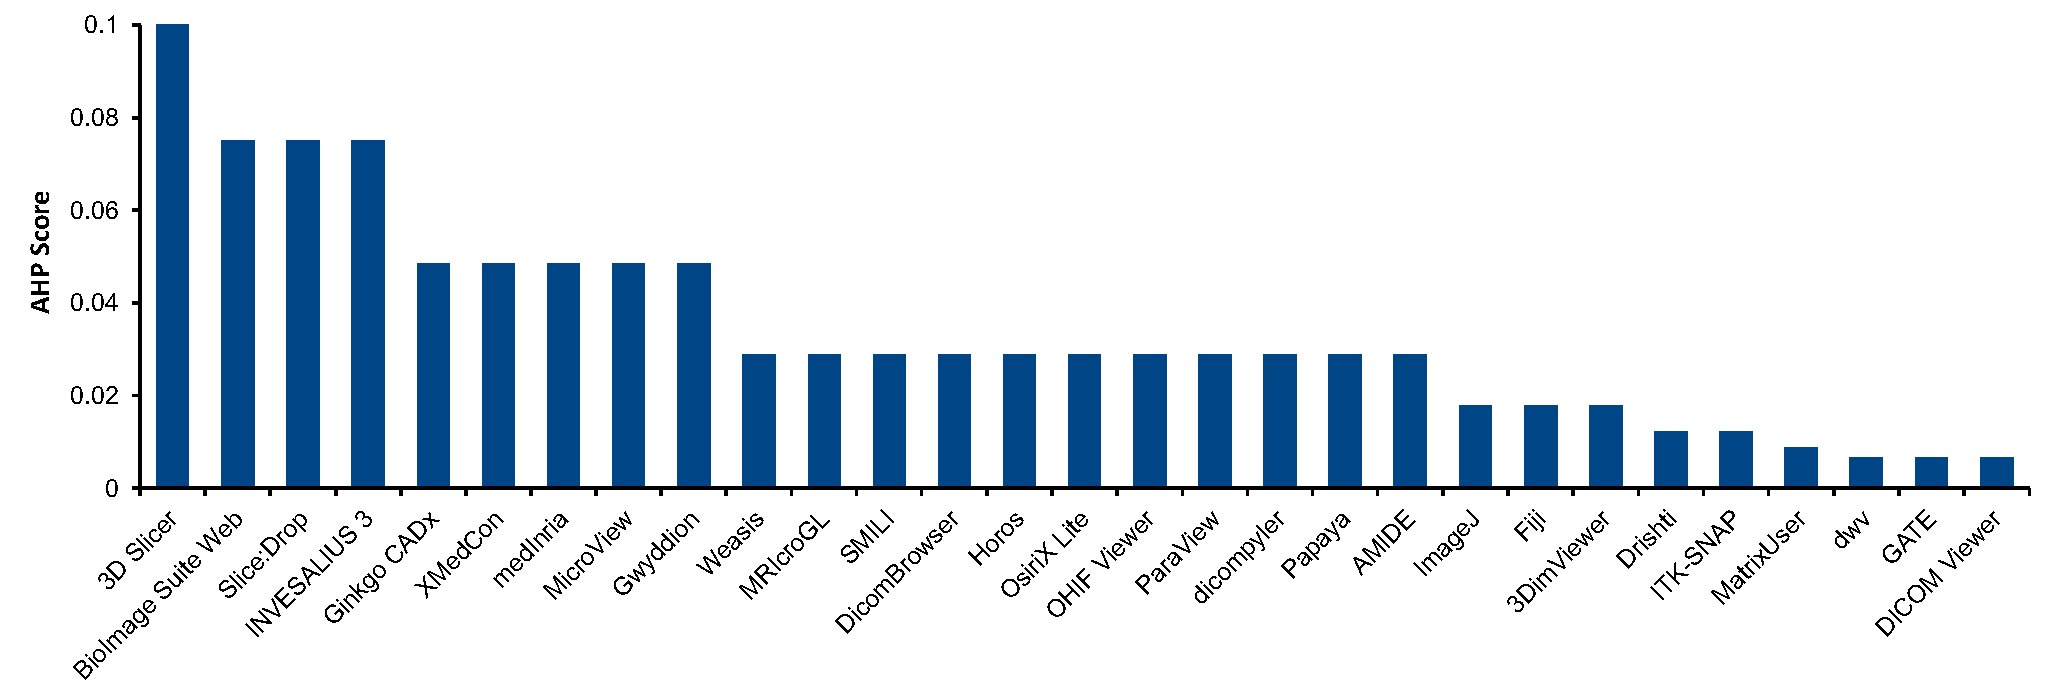
\includegraphics[scale=0.47]{installability_scores.pdf}
\caption{AHP installability scores}
\label{fg_installability_scores}
\end{figure}

\textit{3D Slicer} has the highest score because it had easy to follow
installation instructions, and an automated, fast, frustration-free installation
process. The installer added all dependencies automatically and no errors
occurred during the installation and uninstallation steps. Many other software
packages also had installation instructions and automated installers.  We had no
trouble installing the following packages: \textit{INVESALIUS 3},
\textit{Gwyddion}, \textit{XMedCon}, and \textit{MicroView}. We determined their
scores based on the understandability of the instructions, installation steps,
and user experience. Since \textit{BioImage Suite Web} and \textit{Slice:Drop}
needed no installation, we gave them high scores. \textit{BioImage Suite Web}
also provided an option to download cache for offline usage, which was easy to
apply.

\textit{GATE}, \textit{dwv}, and \textit{DICOM Viewer} showed severe
installation problems. We were not able to install them, even after a reasonable
amount of time (2 hours).  For \textit{dwv} and \textit{GATE} we failed to build
from the source code, but we were able to proceed with measuring other qualities
using a deployed on-line version for \textit{dwv}, and a VM version for
\textit{GATE}. For \textit{DICOM Viewer} we could not install the NextCloud
dependency, and we did not have another option for running the software.
Therefore, for \textit{DICOM Viewer} we could not measure reliability or
robustness.  The other seven qualities could be measured, since they do not
require installation.

\textit{MatrixUser} has a lower score because it depends on Matlab. We assessed
the score from the point of view of a user that would have to install Matlab and
acquire a license.  Of course, for users that already work within Matlab, the
installability score should be higher.

\subsection{Correctness \& Verifiability} \label{sec_result_correctness_verifiability}

Figure~\ref{fg_correctness_verifiability_scores} shows the scores of correctness
and verifiability. Generally speaking, the packages with higher scores adopted
more techniques to improve correctness, and had better documentation for us to
verify against.  For instance, we looked for evidence of unit testing, since it
benefits most parts of the software's life cycle, such as designing, coding,
debugging, and optimization \citep{Hamill2004}.  We only found evidence of unit
testing for about half of the projects. We identified five projects using CI/CD
tools: \textit{3D Slicer}, \textit{ImageJ}, \textit{Fiji}, \textit{dwv}, and
\textit{OHIF Viewer}.

\begin{figure}[!ht]
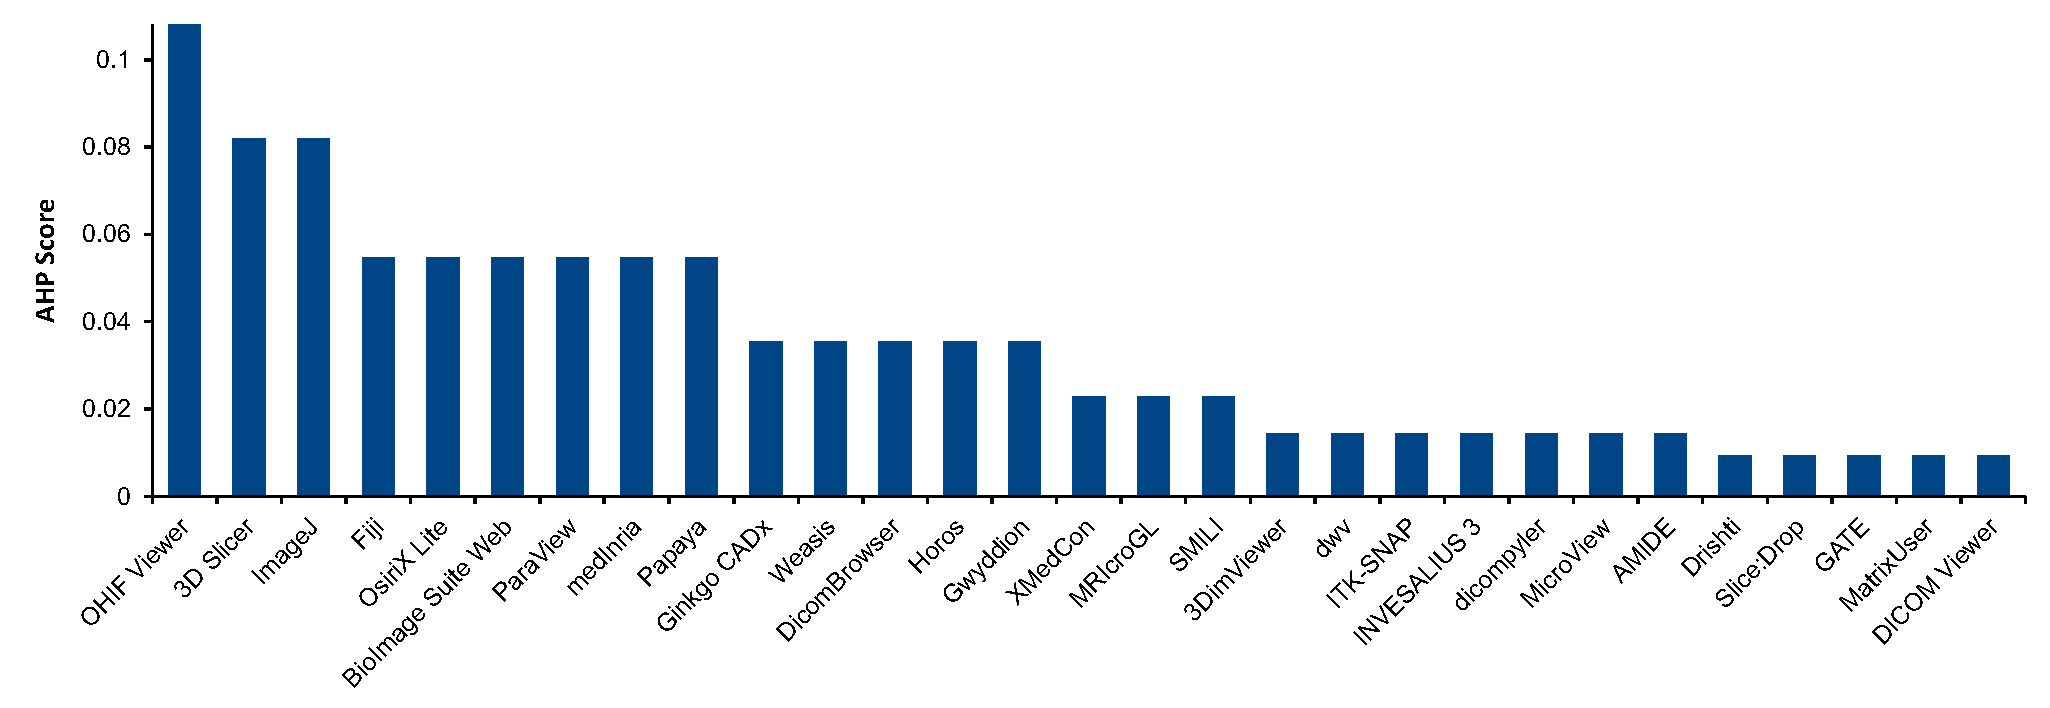
\includegraphics[scale=0.47]{correctness_verifiability_scores.pdf}
\caption{AHP correctness \& verifiability scores}
\label{fg_correctness_verifiability_scores}
\end{figure}

Even for some projects with well-organized documentation, requirements
specifications and theory manuals were still missing.  We could not identify
theory manuals for all projects, and we did not find requirements specifications
for most projects. The only requirements-related document we found was a road
map of \textit{3D Slicer}, which contained design requirements for upcoming
changes.

\subsection{Surface Reliability} \label{sec_result_reliability}

Figure~\ref{fg_reliability_scores} shows the AHP results.  As shown in
Section~\ref{sec_result_installability}, most of the software products did not
``break'' during installation, or did not need installation; \textit{dwv} and
\textit{GATE} broke in the building stage, and the processes were not
recoverable; we could not install the dependency for \textit{DICOM Viewer}. Of
the seven software packages with a getting started tutorial and operation steps
in the tutorial, most showed no error when we followed the steps. However,
\textit{GATE} could not open macro files and became unresponsive several times,
without any descriptive error message. When assessing robustness
(Section~\ref{sec_result_robustness}), we found that \textit{Drishti} crashed
when loading damaged image files, without showing any descriptive error message.
We did not find any problems with the on-line version of
\textit{dwv}.

\begin{figure}[!ht]
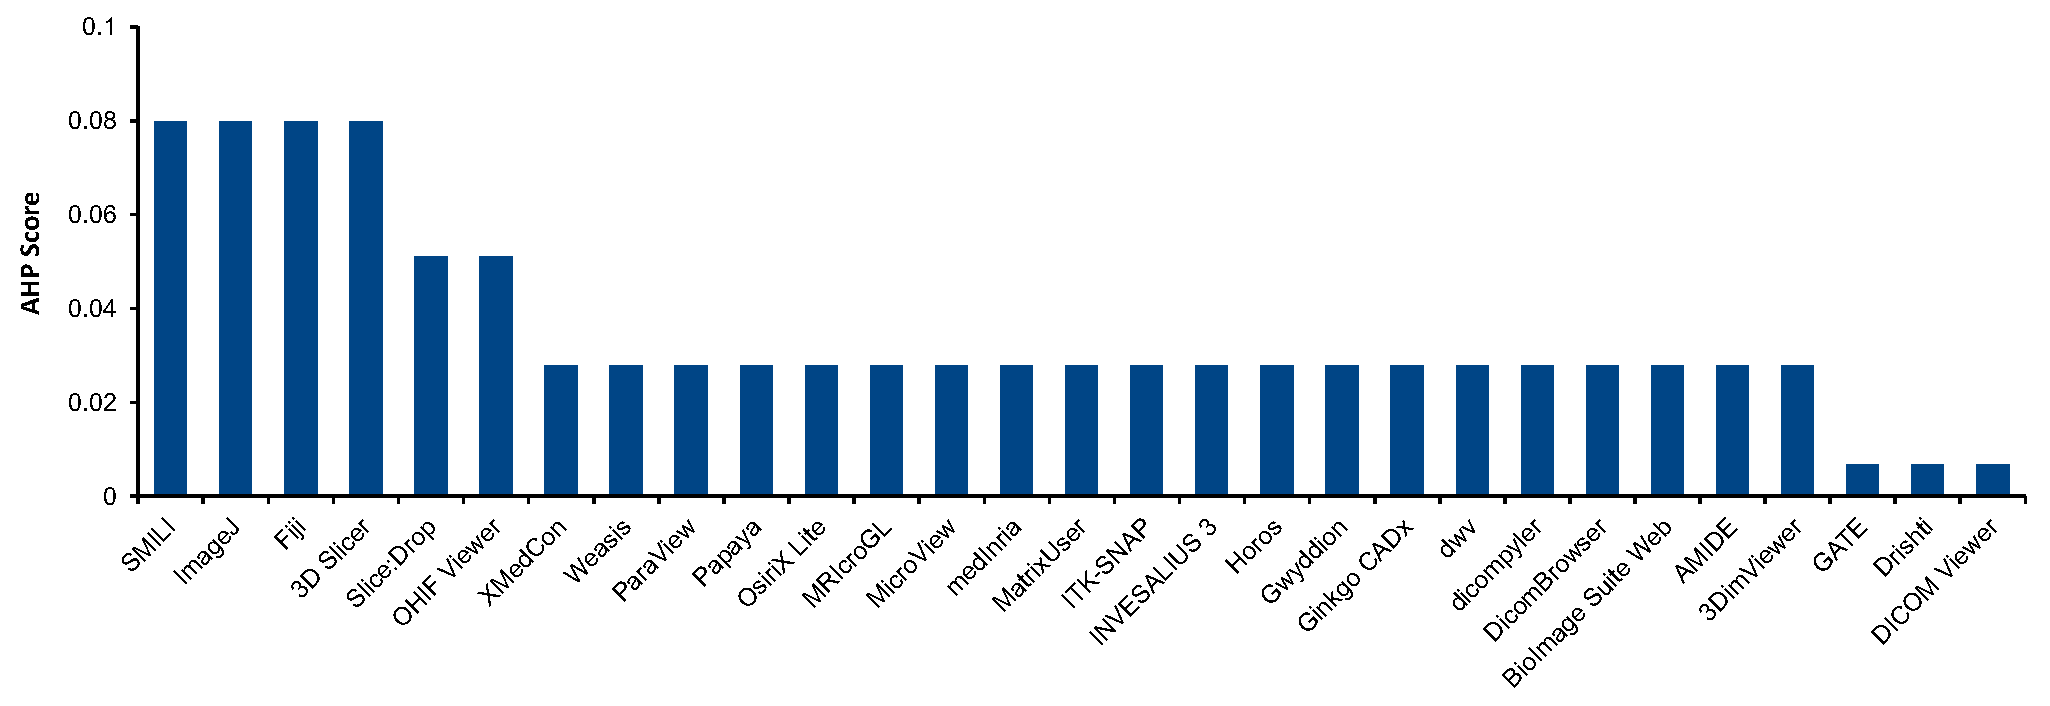
\includegraphics[scale=0.47]{reliability_scores.pdf}
\caption{AHP surface reliability scores}
\label{fg_reliability_scores}
\end{figure}

\subsection{Surface Robustness} \label{sec_result_robustness}

Figure \ref{fg_robustness_scores} presents the scores for surface robustness.
The packages with higher scores elegantly handled unexpected/unanticipated
inputs, typically showing a clear error message. We may have underestimated the
score of \textit{OHIF Viewer}, since we needed further customization to load
data.

\begin{figure}[!ht]
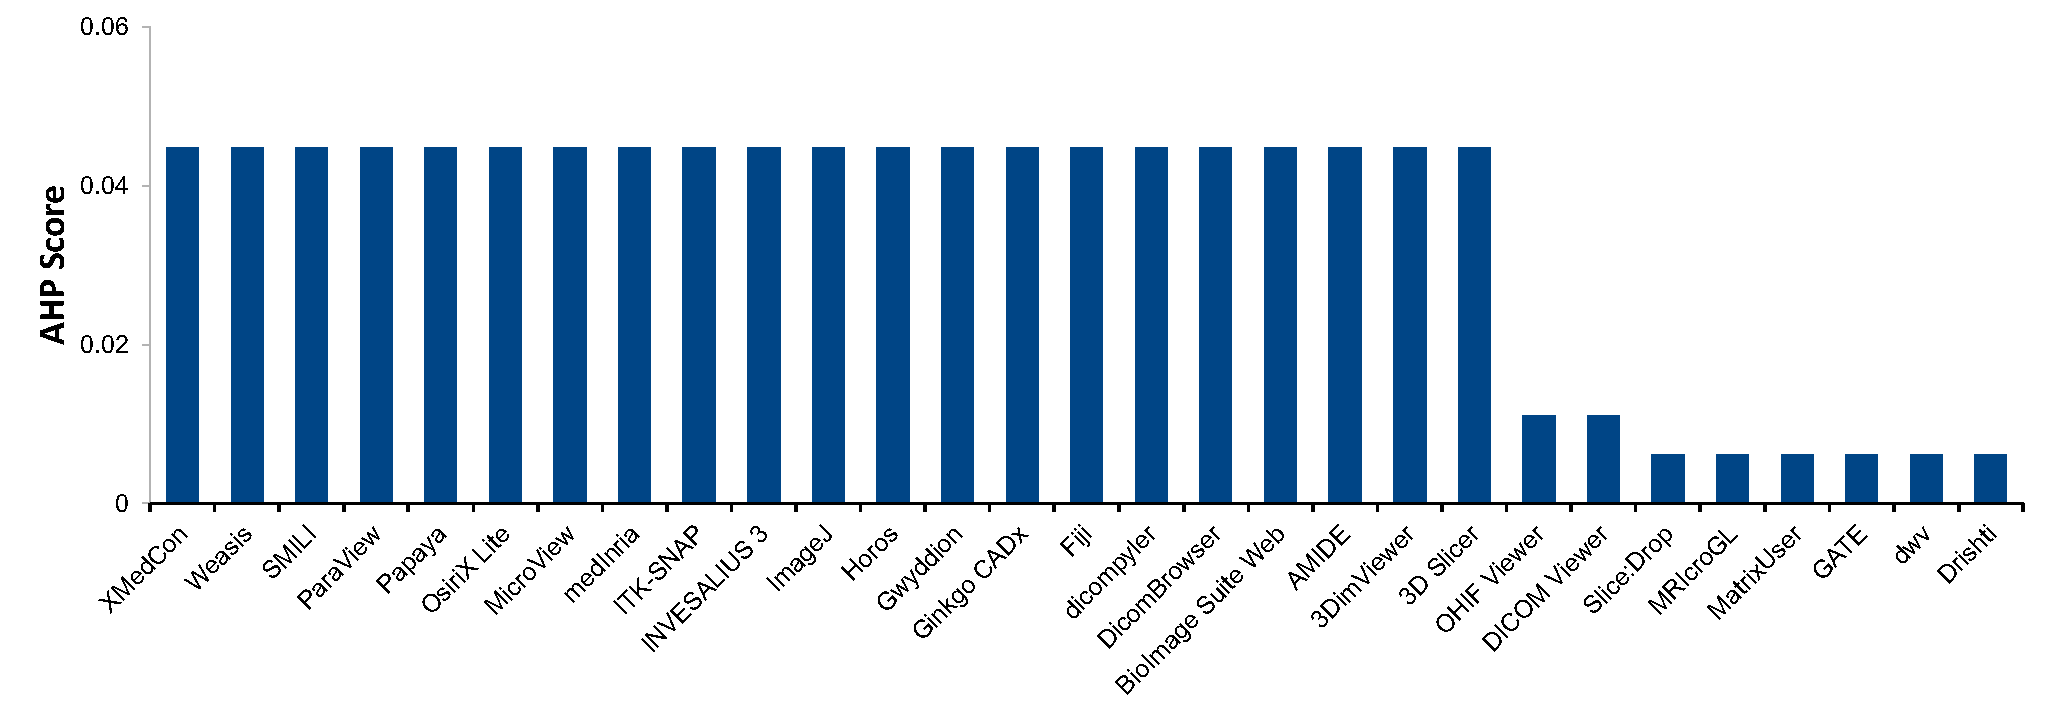
\includegraphics[scale=0.47]{robustness_scores.pdf}
\caption{AHP surface robustness scores}
\label{fg_robustness_scores}
\end{figure}

Digital Imaging and Communications in Medicine (DICOM) ``defines the formats for
medical images that can be exchanged with the data and quality necessary for
clinical use'' \citep{MITA2021}. According to their documentation, all 29
software packages should support the DICOM standard. To test robustness, we
prepared two types of image files: correct and incorrect formats (with the
incorrect format created by relabelled a text file to have the ``.dcm''
extension).  All software packages loaded the correct format image, except for
\textit{GATE}, which failed for unknown reasons.  For the broken format,
\textit{MatrixUser}, \textit{dwv}, and \textit{Slice:Drop} ignored the incorrect
format of the file and loaded it regardless. They did not show any error message
and displayed a blank image. \textit{MRIcroGL} behaved similarly except that it
showed a meaningless image. \textit{Drishti} successfully detected the broken
format of the file, but the software crashed as a result.

\subsection{Surface Usability} \label{sec_result_usability}

Figure~\ref{fg_usability_scores} shows the AHP scores for surface usability. The
software with higher scores usually provided both comprehensive documented
guidance and a good user experience. \textit{INVESALIUS 3} provided an excellent
example of a detailed and precise user manual. \textit{GATE} also provided
numerous documents, but unfortunately we had difficulty understanding and using
them. We found getting started tutorials for only 11 projects, but a user manual
for 22 projects. \textit{MRIcroGL} was the only project that explicitly
documented expected user characteristics.

\begin{figure}[!ht]
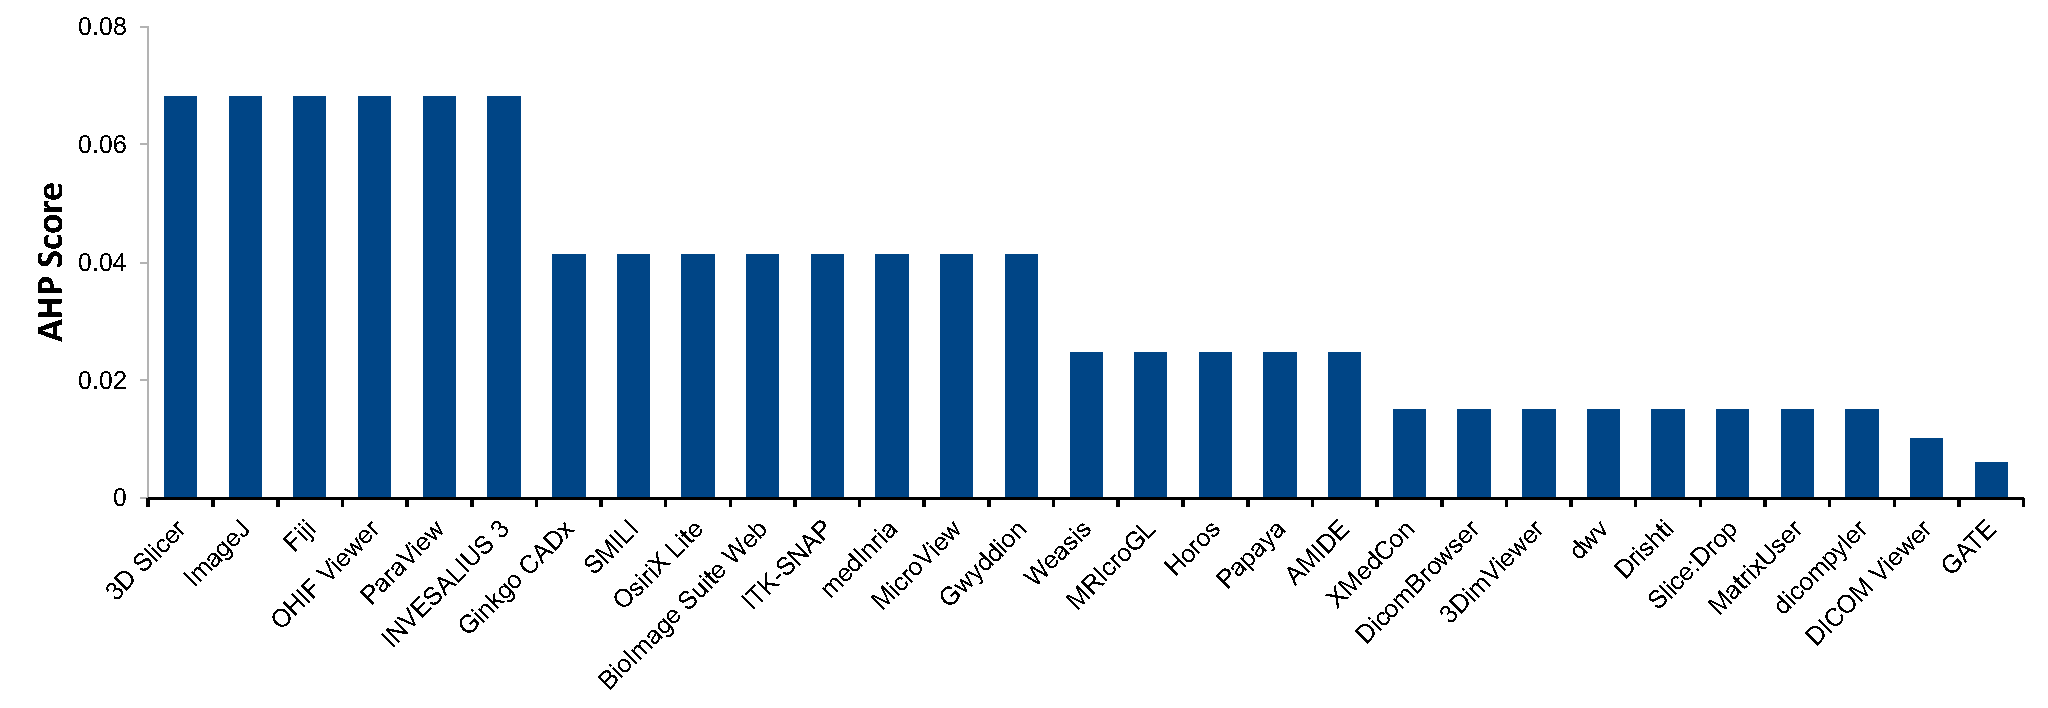
\includegraphics[scale=0.47]{usability_scores.pdf}
\caption{AHP surface usability scores}
\label{fg_usability_scores}
\end{figure}
 
\subsection{Maintainability} \label{sec_score_maintainability}

Figure~\ref{fg_maintainability_scores} shows the ranking results for
maintainability. We gave \textit{3D Slicer} the highest score because we found
it to have the most comprehensive artifacts. For example, as far as we could
find, only a few of the 29 projects had a product, developer's manual, or API
documentation, and only \textit{3D Slicer}, \textit{ImageJ}, \textit{Fiji}
included all three documents. Moreover, \textit{3D Slicer} has a much higher
percentage of closed issues (92\%) compared to \textit{ImageJ} (52\%) and
\textit{Fiji} (64\%). Table~\ref{tab_maintainability_docs} shows which
projects had these documents, in descending order of their maintainability
scores. 

\begin{figure}[!ht]
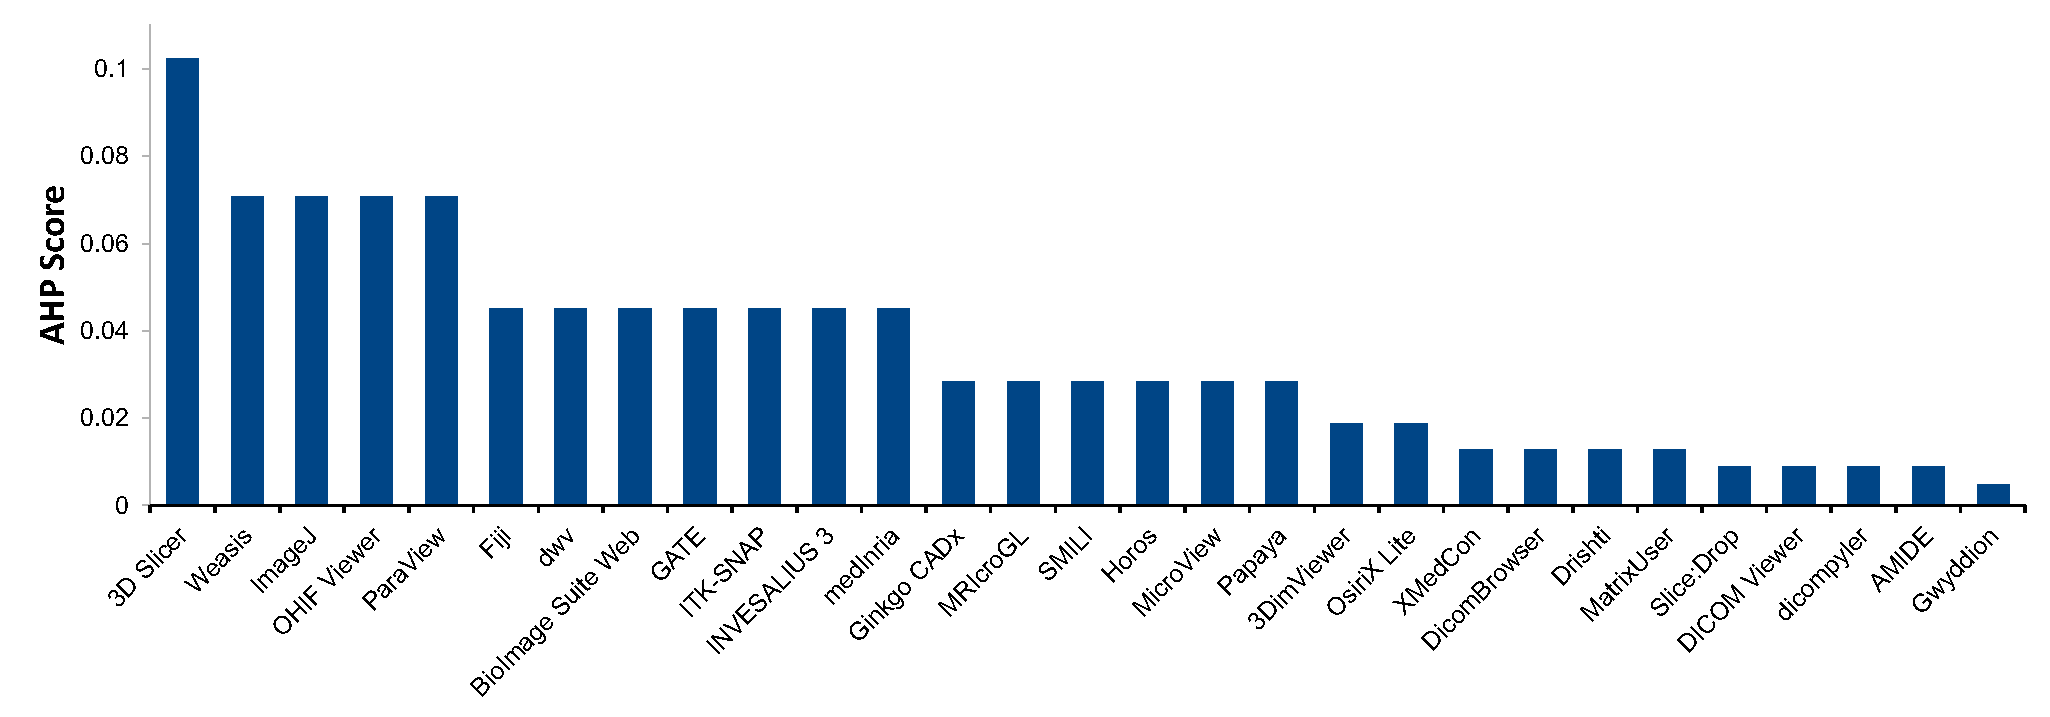
\includegraphics[scale=0.47]{maintainability_scores.pdf}
\caption{AHP maintainability scores}
\label{fg_maintainability_scores}
\end{figure}

\begin{table}[!ht]
\centering
\begin{tabular}{lccc}
\toprule
\multicolumn{1}{c}{Software} & Prod.\ Roadmap & Dev.\ Manual & API Doc. \\ 
\midrule
3D Slicer & \checkmark & \checkmark & \checkmark \\
ImageJ & \checkmark & \checkmark & \checkmark \\
Weasis &  & \checkmark &  \\
OHIF Viewer &  & \checkmark & \checkmark \\
Fiji & \checkmark & \checkmark & \checkmark \\
ParaView & \checkmark &  &  \\
SMILI &  &  & \checkmark \\
medInria &  & \checkmark &  \\
INVESALIUS 3 & \checkmark &  &  \\
dwv &  &  & \checkmark \\
BioImage Suite Web &  & \checkmark &  \\
Gwyddion &  & \checkmark & \checkmark \\ 
\bottomrule
\end{tabular}
\caption{Software with the maintainability documents (listed in descending order of 
maintainability score)}
\label{tab_maintainability_docs}
\end{table}

Twenty-seven of the 29 projects used git as the version control tool, with 24 of these
using GitHub. \textit{AMIDE} used Mercurial and \textit{Gwyddion} used
Subversion. \textit{XMedCon}, \textit{AMIDE}, and \textit{Gwyddion} used
SourceForge. \textit{DicomBrowser} and \textit{3DimViewer} used BitBucket. 

\subsection{Reusability} \label{sec_result_reusability}

Figure~\ref{fg_reusability_scores} shows the AHP results for reusability. As
described in Section~\ref{sec_grading_software}, we gave higher scores to the
projects with API documentation. As shown in
Table~\ref{tab_maintainability_docs}, seven projects had API documents. We also
assumed that projects with more code files and less LOC per code file are more
reusable. Table \ref{tab_loc_per_file} shows the number of text-based files by
project, which we used to approximate the number of code files. The table also
lists the total number of lines (including comments and blanks), LOC, and
average LOC per file. We arranged the items in descending order of their
reusability scores.

\begin{figure}[!ht]
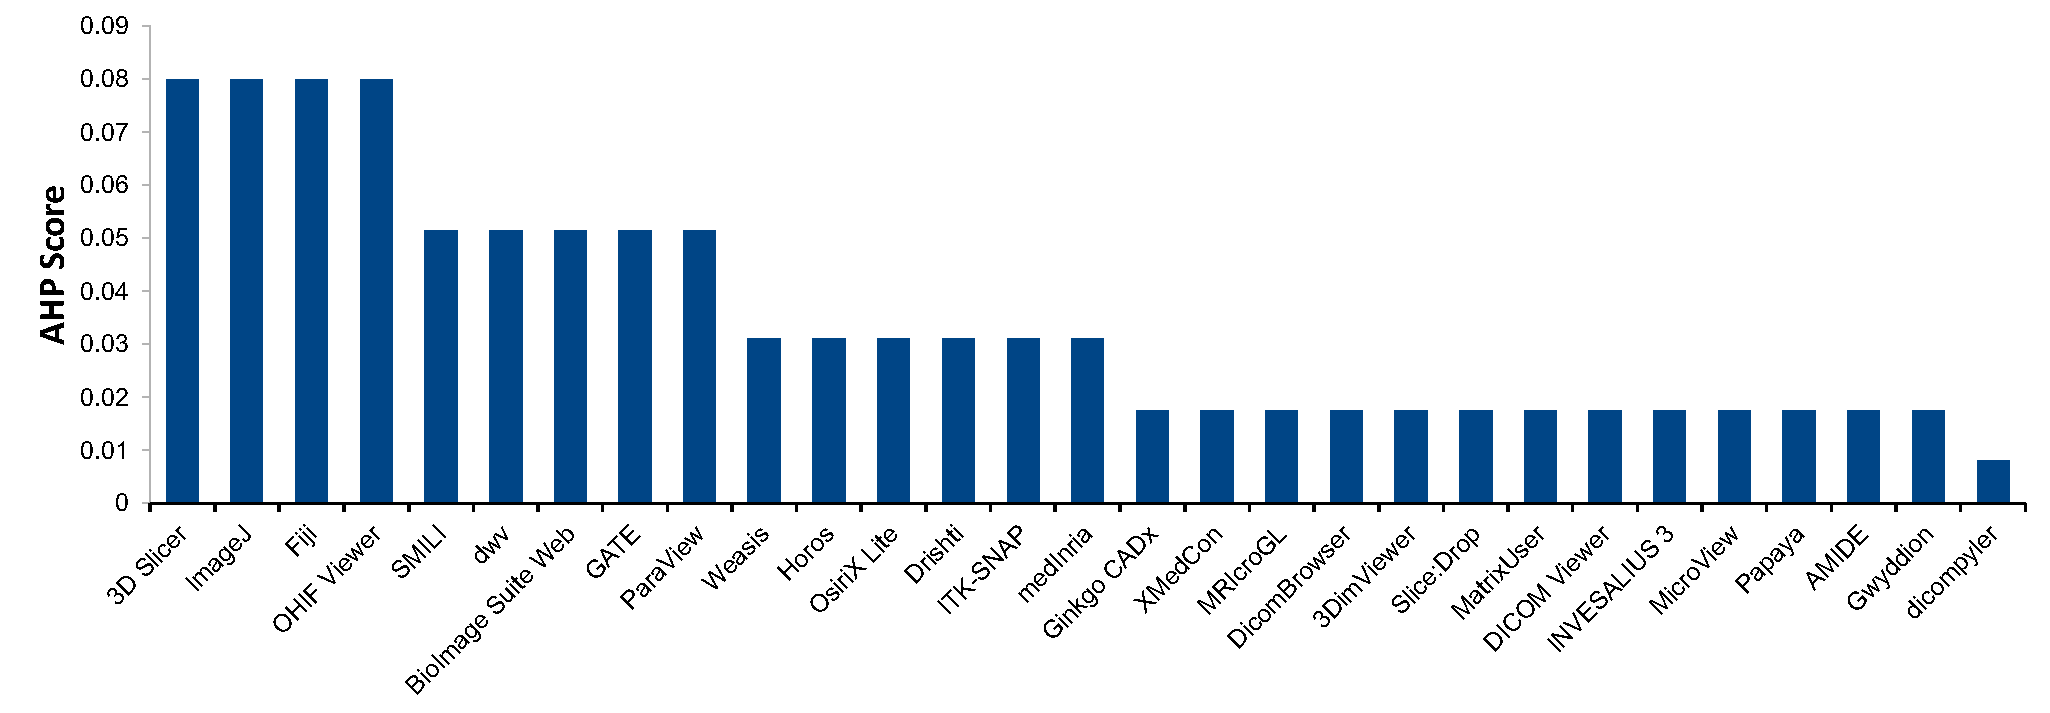
\includegraphics[scale=0.47]{reusability_scores.pdf}
\caption{AHP reusability scores}
\label{fg_reusability_scores}
\end{figure}

\begin{table}[!ht]
\centering
\begin{tabular}{lllll}
\toprule
\multirow{2}{*}{Software} & \multirow{2}{*}{Text Files} & \multirow{2}{*}{Total Lines} & \multirow{2}{*}{LOC} & \multirow{2}{*}{LOC/file} \\
 &  &  &  &  \\ 
\midrule
OHIF Viewer & 1162 & 86306 & 63951 & 55 \\
3D Slicer & 3386 & 709143 & 501451 & 148 \\
Gwyddion & 2060 & 787966 & 643427 & 312 \\
ParaView & 5556 & 1276863 & 886326 & 160 \\
OsiriX Lite & 2270 & 873025 & 544304 & 240 \\
Horos & 2346 & 912496 & 561617 & 239 \\
medInria & 1678 & 214607 & 148924 & 89 \\
Weasis & 1027 & 156551 & 123272 & 120 \\
BioImage Suite Web & 931 & 203810 & 139699 & 150 \\
GATE & 1720 & 311703 & 207122 & 120 \\
Ginkgo CADx & 974 & 361207 & 257144 & 264 \\
SMILI & 275 & 90146 & 62626 & 228 \\
Fiji & 136 & 13764 & 10833 & 80 \\
Drishti & 757 & 345225 & 268168 & 354 \\
ITK-SNAP & 677 & 139880 & 88530 & 131 \\
3DimViewer & 730 & 240627 & 178065 & 244 \\
DICOM Viewer & 302 & 34701 & 30761 & 102 \\
ImageJ & 40 & 10740 & 9681 & 242 \\
dwv & 188 & 71099 & 47815 & 254 \\
MatrixUser & 216 & 31336 & 23121 & 107 \\
INVESALIUS 3 & 156 & 59328 & 48605 & 312 \\
AMIDE & 183 & 139658 & 102827 & 562 \\
Papaya & 110 & 95594 & 71831 & 653 \\
MicroView & 137 & 36173 & 27470 & 201 \\
XMedCon & 202 & 129991 & 96767 & 479 \\
MRIcroGL & 97 & 50445 & 8493 & 88 \\
Slice:Drop & 77 & 25720 & 19020 & 247 \\
DicomBrowser & 54 & 7375 & 5505 & 102 \\
dicompyler & 48 & 19201 & 15941 & 332 \\ 
\bottomrule
\end{tabular}
\caption{Number of files and lines (sorted in descending order of reusability
scores)}
\label{tab_loc_per_file}
\end{table}

\subsection{Surface Understandability} \label{sec_result_understandability}

Figure~\ref{fg_surface_understandability_scores} shows the scores for surface
understandability. All projects had a consistent coding style with parameters in
the same order for all functions; modularized code; and, clear comments, indicating
what is done, not how. However, we only found explicit identification of a
coding standard for 3 out of the 29: \textit{3D Slicer}, \textit{Weasis}, and
\textit{ImageJ}. We also found hard-coded constants (rather than symbolic
constants) in \textit{medInria}, \textit{dicompyler}, \textit{MicroView}, and
\textit{Papaya}. We did not find any reference to the algorithms used in
projects \textit{XMedCon}, \textit{DicomBrowser}, \textit{3DimViewer},
\textit{BioImage Suite Web}, \textit{Slice:Drop}, \textit{MatrixUser},
\textit{DICOM Viewer}, \textit{dicompyler}, and \textit{Papaya}. 

\begin{figure}[!ht]
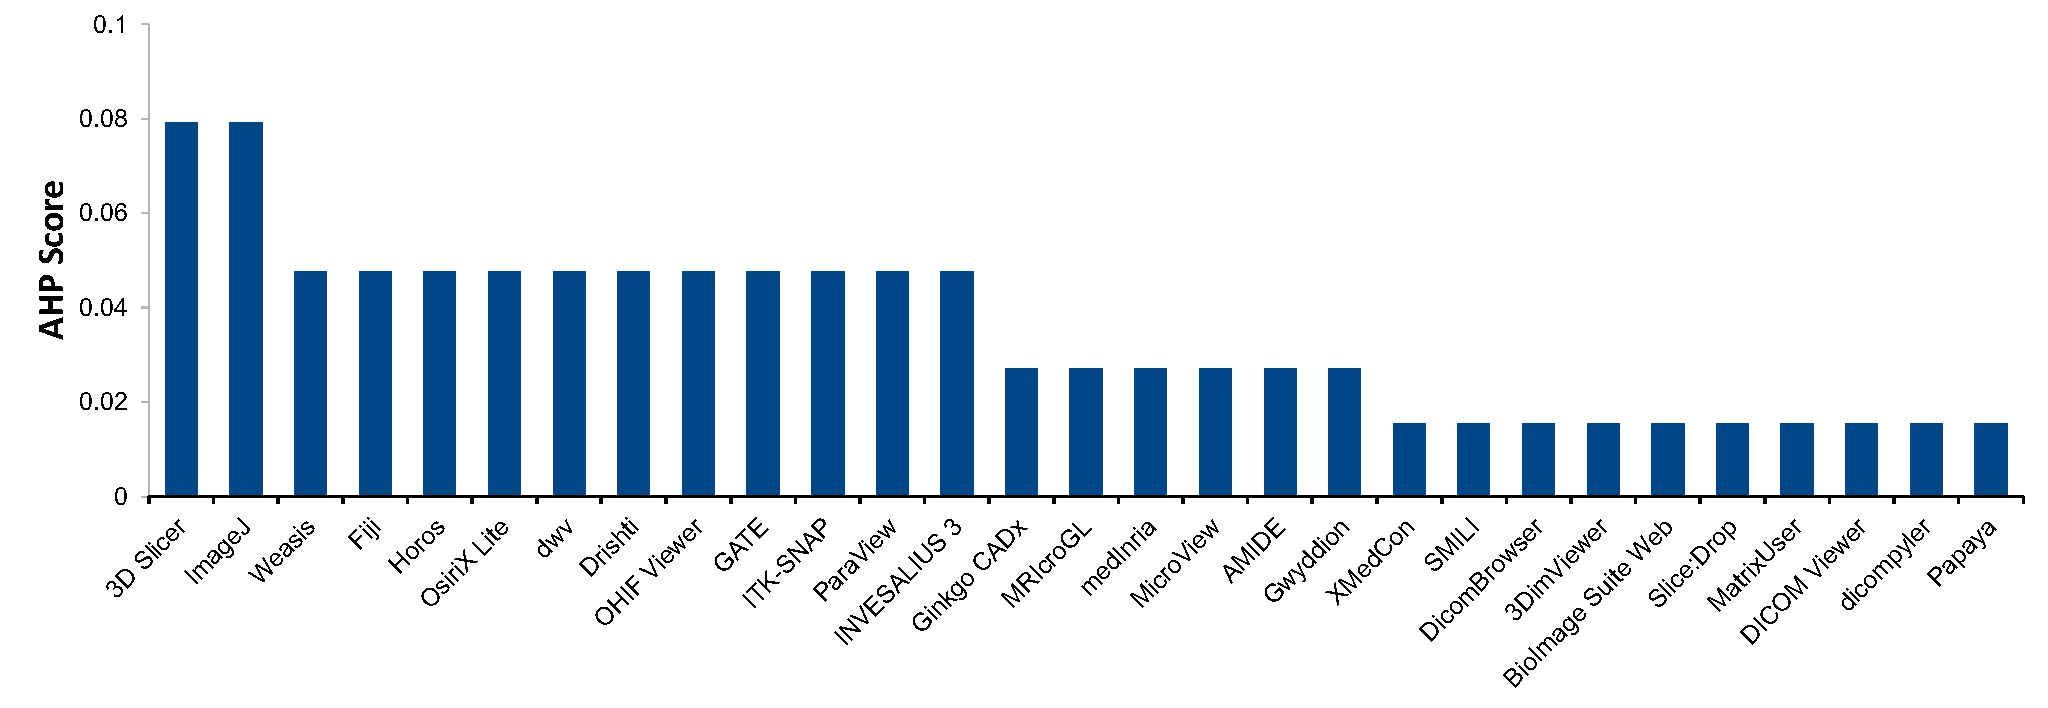
\includegraphics[scale=0.47]{understandability_scores.pdf}
\caption{AHP surface understandability scores}
\label{fg_surface_understandability_scores}
\end{figure}

\subsection{Visibility/Transparency} \label{sec_result_visibility_transparency}

Figure~\ref{fg_visibility_transparency_scores} shows the AHP scores for
visibility/transparency. Generally speaking, the teams that actively documented
their development process and plans scored higher.
Table~\ref{tab_Visibility/Transparency_docs} shows the projects that had
documents for the development process, project status, development environment,
and release notes, in descending order of their visibility/transparency
scores.

\begin{figure}[!ht]
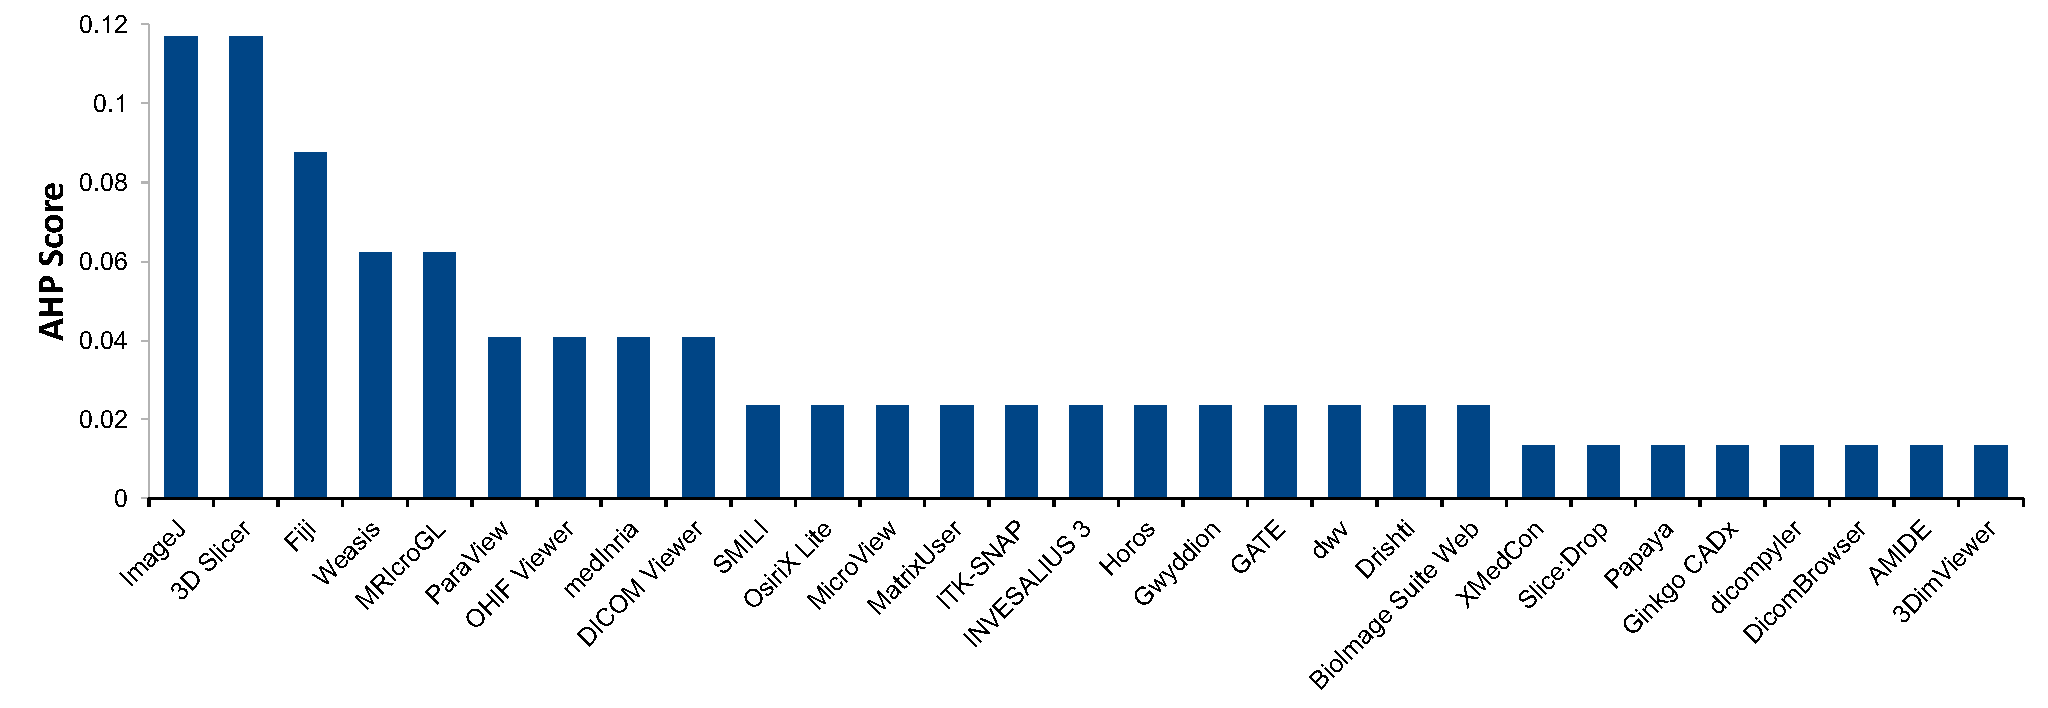
\includegraphics[scale=0.47]{visibility_transparency_scores.pdf}
\caption{AHP visibility/transparency scores}
\label{fg_visibility_transparency_scores}
\end{figure}

\begin{table}[!ht]
\centering
\begin{tabular}{lllll}
\toprule
Software & Dev.\ Process & Proj.\ Status & Dev.\ Env. & Rls.\ Notes \\ 
\midrule
3D Slicer & \checkmark & \checkmark & \checkmark & \checkmark \\
ImageJ & \checkmark & \checkmark & \checkmark & \checkmark \\
Fiji & \checkmark & \checkmark & \checkmark &  \\
MRIcroGL &  &  &  & \checkmark \\
Weasis &  &  & \checkmark & \checkmark \\
ParaView &  & \checkmark &  &  \\
OHIF Viewer &  &  & \checkmark & \checkmark \\
DICOM Viewer &  &  & \checkmark & \checkmark \\
medInria &  &  & \checkmark & \checkmark \\
SMILI &  &  &  & \checkmark \\
Drishti &  &  &  & \checkmark \\
INVESALIUS 3 &  &  &  & \checkmark \\
OsiriX Lite &  &  &  & \checkmark \\
GATE &  &  &  & \checkmark \\
MicroView &  &  &  & \checkmark \\
MatrixUser &  &  &  & \checkmark \\
BioImage Suite Web &  &  & \checkmark &  \\
ITK-SNAP &  &  &  & \checkmark \\
Horos &  &  &  & \checkmark \\
dwv &  &  &  & \checkmark \\
Gwyddion &  &  &  & \checkmark \\ 
\bottomrule
\end{tabular}
\caption{Software with visibility/transparency related documents (listed in
descending order of visibility/transparency score)}
\label{tab_Visibility/Transparency_docs}
\end{table}

\subsection{Overall Scores} \label{Sec_OverallQ}

As described in Section~\ref{sec_AHP}, for our AHP measurements, we have nine
criteria (qualities) and 29 alternatives (software packages). In the absence of
a specific real world context, we assumed all nine qualities are equally
important. Figure~\ref{fg_overall_scores} shows the overall scores in descending
order. Since we produced the scores from the AHP process, the total sum of the
29 scores is precisely 1.0.

\begin{figure}[!ht]
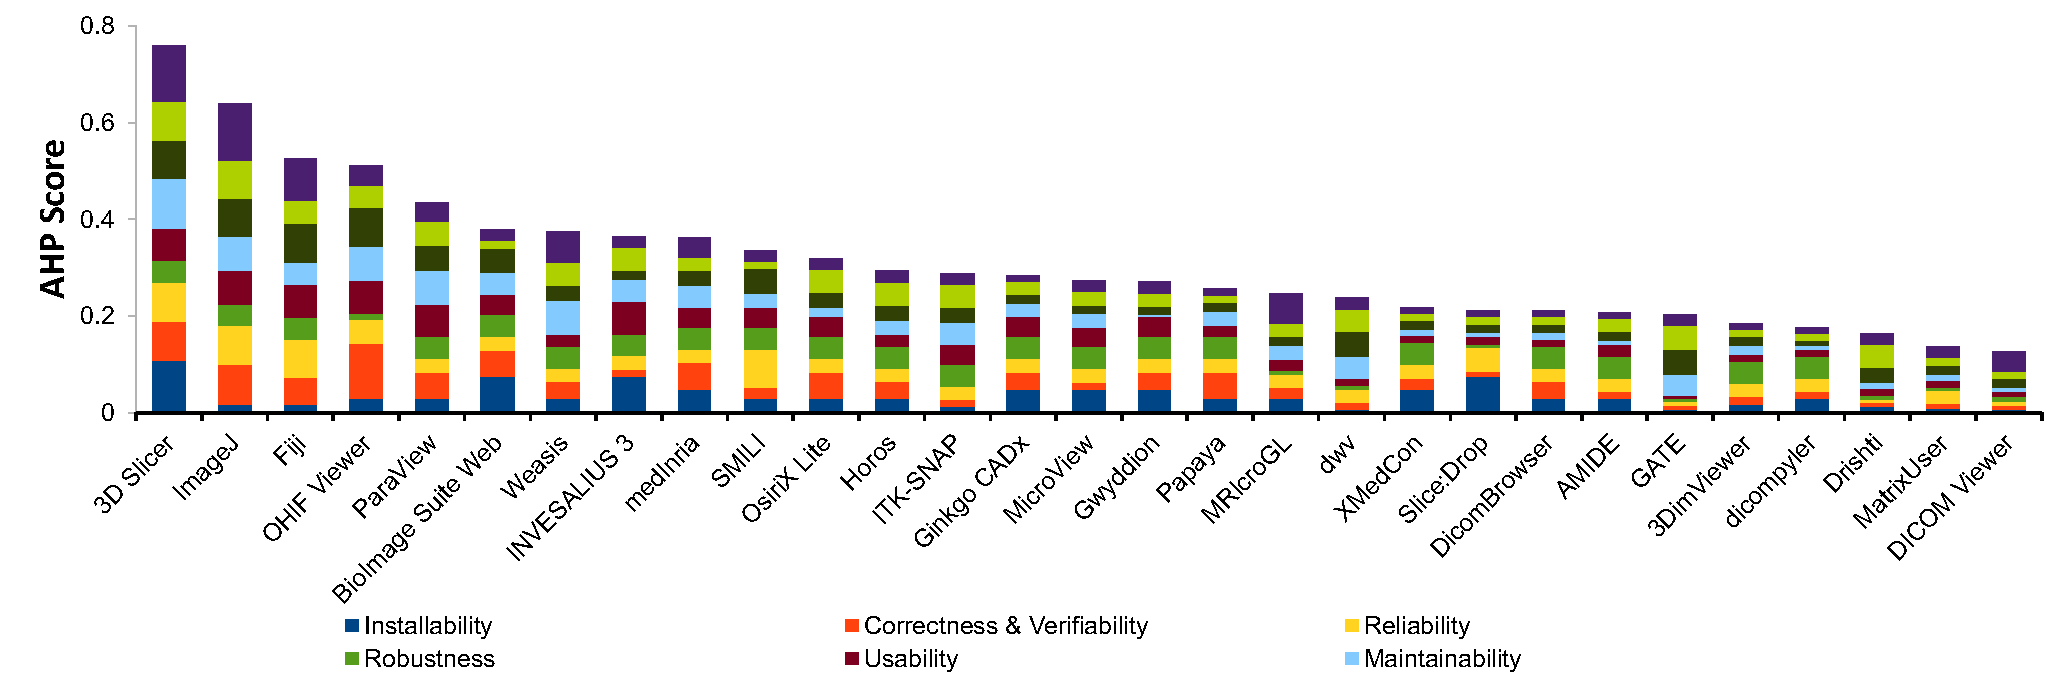
\includegraphics[scale=0.47]{overall_scores.pdf}
\caption{Overall AHP scores with an equal weighting for all 9 software qualities}

\label{fg_overall_scores}
\end{figure}

The top four software products \textit{3D Slicer}, \textit{ImageJ},
\textit{Fiji}, and \textit{OHIF Viewer} have higher scores in most criteria.
\textit{3D Slicer} has a score in the top two for all qualities; \textit{ImageJ}
ranks near the top for all qualities, except for correctness \& verifiability.
\textit{OHIF Viewer} and \textit{Fiji} have similar overall scores, with
\textit{Fiji} doing better in installability and \textit{OHIF Viewer} doing
better in correctness \& verifiability.  Given the installation problems, we may
have underestimated the scores on reliability and robustness for \textit{DICOM
Viewer}, but we compared it equally for the other seven qualities.

\section{Comparison to Community Ranking} \label{Sec_VsCommunityRanking}

To address~\rqref{RQ_CompareHQ2Popular} about how our ranking compares to the
popularity of projects as judged by the scientific community, we make two
comparisons:
\begin{itemize}
\item A comparison of our ranking (from Section~\ref{ch_results}) with the
community ratings on GitHub, as shown by GitHub stars, number of forks, and
number of people watching the projects; and,
\item A comparison of top-rated software from our methodology with the top
recommendations from our domain experts (as mentioned in
Section~\ref{sec_software_selection}).
\end{itemize}

Table~\ref{tab_ranking_vs_GitHub} shows our ranking of the 29 MI projects, and
their GitHub metrics, if applicable. As mentioned in
Section~\ref{sec_score_maintainability}, 24 projects used GitHub. Since GitHub
repositories have different creation dates, we collect the number of months each
stayed on GitHub, and calculate the average number of new stars, people
watching, and forks per 12 months. Section~\ref{sec_grading_software} describes
the method of getting the creation date.  The items in
Table~\ref{tab_ranking_vs_GitHub} are listed in descending order of the average
number of new stars per year.  The non-GitHub items are listed in the order of
our ranking.  We collected all GitHub statistics in July 2021.  

Generally speaking, most of the top-ranking MI software projects also received
greater attention and popularity on GitHub. Between our ranking and the GitHub
stars-per-year ranking, four of the top five software projects appear in both
lists. Our top five packages are scattered among the first eight positions on the
GitHub list. However, as discussed below there are discrepancies between the two
lists.

In some cases projects are popular in the community, but were assigned a low
rank by our methodology.  This is the case for \textit{dwv}. The reason for the
low ranking is that, as mentioned in Section~\ref{sec_result_installability}, we
failed to build it locally, and used the test version on its websites for the
measurements. We followed the instructions and tried to run the command ``yarn
run test'' locally, which did not work. In addition, the test version did not
detect a broken DICOM file and displayed a blank image as described in
Section~\ref{sec_result_robustness}. We might underestimate the scores for
\textit{dwv} due to uncommon technical issues. 

We also ranked \textit{DICOM Viewer} much lower than its popularity. As
mentioned in Section~\ref{sec_result_installability}, it depended on the
NextCloud platform that we could not successfully install. Thus, we might
underestimate the scores of its surface reliability and surface robustness. 

Further reason for discrepancies between our ranking and the community's ranking
is that we weighted all qualities equally. This is not likely how users
implicitly rank the different qualities. As a result, some projects with high
community popularity may have scored lower with our method because of a
relatively higher (compared to the scientific community's implicit ranking)
weighting of the poor scores for some qualities. A further explanation for
discrepancies between our measures and the star measures may also be due to
inaccuracy with using stars to approximate popularity.  Stars are not an ideal
measure because stars represent the community's feeling in the past more than
they measure current preferences \citep{Szulik2017}.  The issue with stars is
that they tend only to be added, not removed.  A final reason for
inconsistencies between our ranking and the community's ranking is that, as for
consumer products, more factors influence popularity than just quality.

\begingroup
\renewcommand{\arraystretch}{0.85}
\begin{table}[!ht]
\centering
\begin{tabular}{llllll}
\toprule
Software & Comm.\ Rank & Our Rank & Stars/yr & Watches/yr & Forks/yr \\ 
\midrule
3D Slicer & 1 & 1 & 284 & 19 & 128 \\
OHIF Viewer & 2 & 4 & 277 & 19 & 224 \\
dwv & 3 & 19 & 124 & 12 & 51 \\
ImageJ & 4 & 2 & 84 & 9 & 30 \\
ParaView & 5 & 5 & 67 & 7 & 28 \\
Horos & 6 & 12 & 49 & 9 & 18 \\
Papaya & 7 & 17 & 45 & 5 & 20 \\
Fiji & 8 & 3 & 44 & 5 & 21 \\
DICOM Viewer & 9 & 29 & 43 & 6 & 9 \\
INVESALIUS 3 & 10 & 8 & 40 & 4 & 17 \\
Weasis & 11 & 7 & 36 & 5 & 19 \\
dicompyler & 12 & 26 & 35 & 5 & 14 \\
OsiriX Lite & 13 & 11 & 34 & 9 & 24 \\
MRIcroGL & 14 & 18 & 24 & 3 & 3 \\
GATE & 15 & 24 & 19 & 6 & 26 \\
Ginkgo CADx & 16 & 14 & 19 & 4 & 6 \\
BioImage Suite Web & 17 & 6 & 18 & 5 & 7 \\
Drishti & 18 & 27 & 16 & 4 & 4 \\
Slice:Drop & 19 & 21 & 10 & 2 & 5 \\
ITK-SNAP & 20 & 13 & 9 & 1 & 4 \\
medInria & 21 & 9 & 7 & 3 & 6 \\
SMILI & 22 & 10 & 3 & 1 & 2 \\
MatrixUser & 23 & 28 & 2 & 0 & 0 \\
MicroView & 24 & 15 & 1 & 1 & 1 \\
Gwyddion & 25 & 16 & n/a & n/a & n/a \\
XMedCon & 26 & 20 & n/a & n/a & n/a \\
DicomBrowser & 27 & 22 & n/a & n/a & n/a \\
AMIDE & 28 & 23 & n/a & n/a & n/a \\
3DimViewer & 29 & 25 & n/a & n/a & n/a \\ 
\bottomrule
\end{tabular}
\caption{Software ranking by our methodology versus the community (Comm.)\
ranking using GitHub metrics (Sorted in descending order of community
popularity, as estimated by the number of new stars per year)}
\label{tab_ranking_vs_GitHub}
\end{table}
\endgroup

As shown in Section~\ref{sec_software_selection}, our domain experts recommended
a list of top software with 12 software products.  All the top 4 entries from
the Domain Expert's list are among the top 12 ranked by our methodology. Three
of the top four on both lists are the same: \textit{3D Slicer}, \textit{ImageJ},
and \textit{Fiji}. \textit{3D Slicer} is top project by both rankings (and by
the GitHub stars measure as well).  The Domain Expert ranked \textit{Horos} as
their second choice, while we ranked it twelfth.  Our third ranked project,
\textit{OHIF Viewer} was not listed by the Domain Expert.  Neither were the
software packages that we ranked from fifth to eleventh (\textit{ParaView},
\textit{Weasis}, \textit{medInria}, \textit{BioImage Suite Web}, \textit{OsiriX
Lite}, \textit{INVESALIUS}, and \textit{Gwyddion}).  The software mentioned by
the Domain Expert that we did not rank were the six recommended packages that
did not have visualization as the primary function (as discussed in
Section~\ref{sec_software_selection}).  The differences between the list
recommended by our methodology and the Domain Expert are not surprising.  As
mentioned above, our methodology weights all qualities equally, but that may not
be the case for the Domain Expert's impressions.  Moreover, although the Domain
Expert has significant experience with MI software, they have not used all 29
packages that were measured.

Although our ranking and the estimate of the community's ranking are not perfect
measures, they do suggest a correlation between best practices and popularity.
We do not know which comes first, the use of best practices or popularity, but
we do know that the top ranked packages tend to incorporate best practices. The
next sections will explore how the practices of the MI community compare to the
broader research software community. We will also investigate the practices from
the top projects that others within the MI community, and within the broader
research software community, can potentially adopt.

\section{Comparison Between MI and Research Software for Artifacts}
\label{Sec_CompareArtifacts}

As part of filling in the measurement template (from
Section~\ref{sec_grading_software}), we summarized the artifacts observed in
each MI package. Table~\ref{artifactspresent} groups the artifacts by frequency
into categories of common (20 to 29 ($>$67\%) packages), uncommon (10 to 19
(33-67\%) packages), and rare (1 to 9 ($<$33\%) packages). \citet{Dong2021-Data}
summarizes the full measurements.  Tables~\ref{tab_maintainability_docs}
and~\ref{tab_Visibility/Transparency_docs} show the details on which projects
use which types of artifacts for documents related to maintainability and
visibility, respectively.

\begin{table}[ht!]
    \begin{center}
    \begin{tabular}{ p{4.6 cm} p{5.6 cm} p{5 cm}}
    \toprule
    Common & Uncommon & Rare \\
    \midrule
    README (29) & Build scripts (18) & Getting Started (9)\\
    Version control (29) & Tutorials (18) & Developer's manual (8)\\
    License (28) & Installation guide (16) & Contributing (8)\\
    Issue tracker (28) & Test cases (15) & API documentation (7)\\
    User manual (22) & Authors (14) & Dependency list (7)\\
    Release info. (22) & Frequently Asked Questions (FAQ) (14) & Troubleshooting guide (6)\\
     & Acknowledgements (12) & Product roadmap (5)\\
     & Changelog (12) & Design documentation (5)\\
     & Citation (11) & Code style guide (3)\\
     & & Code of conduct (1)\\
     & & Requirements (1)\\
    \bottomrule
    \end{tabular}
    \caption{Artifacts Present in MI Packages, Classified by Frequency (The number 
    in brackets is the number of occurrences)}
    \label{artifactspresent}
    \end{center}
\end{table}

We answer~\rqref{RQ_CompareArtifacts} by comparing the artifacts that we
observed in MI repositories to those observed and recommended for research
software in general. Our comparison may point out areas where some MI software
packages fall short of current best practices. This is not intended to be a
criticism of any existing packages, especially since in practice not every
project needs to achieve the highest possible quality. However, rather than
delve into the nuances of which software can justify compromising which
practices we will write our comparison under the ideal assumption that every
project has sufficient resources to match best practices.
    
Table~\ref{Tbl_Guidelines} (based on data from \citep{SmithAndMichalski2022})
shows that MI artifacts generally match the recommendations found in nine
current research software development guidelines:
\begin{itemize}
\item United States Geological Survey Software Planning Checklist
\citep{USGS2019},
\item DLR (German Aerospace Centre) Software Engineering Guidelines
\citep{TobiasEtAl2018}, 
\item Scottish Covid-19 Response Consortium Software Checklist
\citep{BrettEtAl2021},
\item Good Enough Practices in Scientific Computing \citep{WilsonEtAl2016},
\item xSDK (Extreme-scale Scientific Software Development Kit) Community Package
Policies \citep{SmithAndRoscoe2018},
\item Trilinos Developers Guide \citep{HerouxEtAl2008},
\item EURISE (European Research Infrastructure Software Engineers') Network
Technical Reference \citep{ThielEtAl2020},
\item CLARIAH (Common Lab Research Infrastructure for the Arts and Humanities)
Guidelines for Software Quality \citep{vanGompelEtAl2016}, and
\item A Set of Common Software Quality Assurance Baseline Criteria for Research
Projects \citep{OrvizEtAl2017}.
\end{itemize}

In Table~\ref{Tbl_Guidelines} each row corresponds to an artifact.  For a given
row, a checkmark in one of the columns means that the corresponding guideline
recommends this artifact.  The last column shows whether the artifact appears in
the measured set of MI software, either not at all (blank), commonly (C),
uncommonly (U) or rarely (R).  We did our best to interpret the meaning of each
artifact consistently between guidelines and specific MI software, but the
terminology and the contents of artifacts are not standardized.  The challenge
even exists for the ubiquitous README file.  As illustrated by
\citet{PranaEtAl2018}, the content of README files shows significant variation
between projects.  Although some content is reasonably consistent, with 97\% of
README files contain at least one section describing the `What' of the
repository and 89\% offering some `How' content, other categories are more
variable.  For instance, information on `Contribution', `Why', and `Who',
appear in 28\%, 26\% and 53\% of the analyzed files, respectively
\citep{PranaEtAl2018}.  

The frequency of checkmarks in Table~\ref{Tbl_Guidelines} indicates the
popularity of recommending a given artifact, but it does not imply that the most
commonly recommended artifacts are the most important artifacts. Just because a
guideline does not explicitly recommend an artifact, does not mean the guideline
authors do not value that artifact.  They may have excluded it because it is out
of the scope of their recommendations, or outside their experience.  For
instance, an artifact related to uninstall is only explicitly mentioned by
\citet{vanGompelEtAl2016}, but other guideline authors would likely see its
value.  They may simply feel that uninstall is implied by install, or they may
have never asked themselves whether they need separate uninstall instructions.

\begin{table}[H]
\begin{center}
\begin{tabular}{ p{2.5cm}p{1cm}p{1cm}p{1cm}p{1cm}p{1cm}p{1cm}p{1cm}p{1.2cm}p{1cm}p{0.8cm} }
\toprule
~ \ & \citet{USGS2019} & \citet{TobiasEtAl2018} & \citet{BrettEtAl2021} &
\citet{WilsonEtAl2016} & \citet{SmithAndRoscoe2018} & \citet{HerouxEtAl2008} &
\citet{ThielEtAl2020} & \citet{vanGompelEtAl2016} & \citet{OrvizEtAl2017} & MI\\
\midrule
LICENSE & \checkmark & \checkmark & \checkmark & \checkmark & \checkmark & &
\checkmark & \checkmark & \checkmark & C\\
README &  & \checkmark & \checkmark & \checkmark & \checkmark & & \checkmark &
\checkmark & \checkmark & C\\
CONTRIBUTING &  & \checkmark & \checkmark & \checkmark & \checkmark & &
\checkmark & \checkmark & \checkmark & R\\
CITATION &  &  &  & \checkmark & & & & \checkmark & \checkmark & U\\
CHANGELOG &  & \checkmark &  & \checkmark & \checkmark & & \checkmark &  &  & U\\
INSTALL &  &  &  &  & \checkmark & & \checkmark & \checkmark & \checkmark & U\\
\midrule
Uninstall &  &  &  &  & & & & \checkmark & &  \\
Dependency List &  &  & \checkmark & & \checkmark & & & \checkmark &  & R\\
Authors &  &  &  &  &  &  & \checkmark & \checkmark & \checkmark & U\\
Code of Conduct &  &  &  &  & & & \checkmark & & & R\\
Acknowledgements &  &  &  &  &  &  & \checkmark & \checkmark & \checkmark & U\\
Code Style Guide &  & \checkmark &  &  & & & \checkmark & \checkmark & \checkmark & R\\
Release Info. &  & \checkmark &  &  & & \checkmark & \checkmark & & & C\\
Prod.\ Roadmap &  &  &  &  & & \checkmark & \checkmark & \checkmark & & R\\
\midrule
Getting started &  &  &  &  & \checkmark & & \checkmark & \checkmark & \checkmark & R\\
User manual &  &  & \checkmark &  & & & \checkmark & & & C\\
Tutorials &  &  &  &  & & & \checkmark & & & U\\
FAQ &  &  &  &  & & & \checkmark & \checkmark & \checkmark & U\\
\midrule
Issue Track &  & \checkmark & \checkmark & & \checkmark & \checkmark &
\checkmark & & \checkmark & C\\
Version Control &  & \checkmark & \checkmark & \checkmark & \checkmark &
\checkmark & \checkmark & \checkmark & \checkmark & C\\ 
Build Scripts &  & \checkmark &  & \checkmark & \checkmark & \checkmark &
\checkmark & & \checkmark & U\\
\midrule
Requirements &  & \checkmark &  &  & & \checkmark &  &  & \checkmark & R\\
Design Doc.\ &  & \checkmark  & \checkmark &  & \checkmark & & \checkmark &
\checkmark& \checkmark & R\\
API Doc. &  &  &  &  & \checkmark & & \checkmark & \checkmark & \checkmark & R\\
Test Plan &  & \checkmark &  &  & & \checkmark & & & &  \\
Test Cases & \checkmark & \checkmark & \checkmark &  & \checkmark & \checkmark &
\checkmark & \checkmark & \checkmark & U\\
\bottomrule
\end{tabular}
\caption{Comparison of Recommended Artifacts in Software Development Guidelines
to Artifacts in MI Projects (C for Common, U for Uncommon and R for Rare)}
\label{Tbl_Guidelines}
\end{center}
\end{table}

Two of the items that appear in Table~\ref{artifactspresent} do not appear in
the software development guidelines shown in Table~\ref{Tbl_Guidelines}:
Troubleshooting guide and Developer's manual.  Although the guidelines do not
name these two artifacts, the information contained within them overlaps with
the recommended artifacts.  A Troubleshooting guideline contains information
that would typically be found in a User manual.  A Developer's guide overlaps
with information from the README, INSTALL, Uninstall, Dependency List, Release
Information, API documentation and Design documentation.  In our current
analysis, we have identified artifacts by the names given by the software
guidelines and MI examples.  In the future, a more in-depth analysis would look
at the knowledge fragments that are captured in the artifacts, rather than
focusing on the names of the files that collect these fragments together.

Although the MI community shows examples of 88\% (23 of 26) of the practices we
found in research software guidelines (Table~\ref{Tbl_Guidelines}), we did not
observe three recommended artifacts: i) Uninstall, ii) Test plans, and iii)
Requirements.  Uninstall is likely an omission caused by the focus on installing
software. Given the storage capacity of current hardware, developers and users
are not generally concerned with uninstall.  Moreover, as mentioned above,
uninstall is not particularly emphasized in existing recommendations.  

Test plans describe the scope, approach, resources, and the schedule of planned
test activities \citep{VanVliet2000}.  The plan should cover details such as the
makeup of the testing team, automated testing tools and technology to employ,
the testing process, system tests, integration tests and unit tests. We did not
observe test plans for MI software, but that doesn't mean plans weren't created;
it means that the plans are not under version control. Test plans would have to
at least be implicitly created, since we observed test cases with reasonable
frequency for MI software (test cases are categorized as uncommon).

The other apparently neglected document is the requirements specification, which
records the functionalities, expected performance, goals, context, design
constraints, external interfaces and other quality attributes of the software
\citep{IEEE1998}.  If developers write requirements they typically are based on
a template, which provide documentation structure, guidelines, and rules.
Although there is no universally accepted template, examples include
\citet{ESA1991}, \citet{IEEE1998}, \citet{NASA1989}, and
\citet{RobertsonAndRobertson1999Vol}.

MI software is like other research software in its neglect of requirements
documentation.  Although requirements documentation is recommended by some
\citep{TobiasEtAl2018, HerouxEtAl2008, SmithAndKoothoor2016}, in practice
research software developers often do not produce a proper requirements
specification \citep{HeatonAndCarver2015}. \citet{SandersAndKelly2008}
interviewed 16 scientists from 10 disciplines and found that none of the
scientists created requirements specifications, unless regulations in their
field mandated such a document. \citet{Nguyen-HoanEtAl2010} showed requirements
are the least commonly produced type of documentation for research software in
general. When looking at the pain points for research software developers,
\citet{WieseEtAl2019} found that software requirements and management is the
software engineering discipline that most hurts scientific developers,
accounting for 23\% of the technical problems reported by study participants.
The lack of support for requirements is likely due to the perception that
up-front requirements are impossible for research software
\citep{CarverEtAl2007, SegalAndMorris2008}, but if we drop the insistence on
``up-front'' requirements, allowing instead for the requirements to be written
iteratively and incrementally, requirements are feasible \citep{Smith2016}.
\citet{SmithEtAl2007} provides a requirements template tailored to research
software. 

Table~\ref{Tbl_Guidelines} shows several recommended artifacts that are rarely
observed in practice.  A theme among these rare artifacts is that, except for
the user-focused getting started manual, they are developer-focused.  The
dependency list, which is a list of software library dependencies, was rarely
observed, but this information is still likely present, just embedded in build
scripts. The other developer-focused and rare artifacts are as follows:

\begin{itemize}

\item \textbf{A Contributing file} provides new contributors with the information
that they need to start adding/modifying the repository's files.
\citet{Abdalla2016} provides a simple template for creating an open-source
contributor guideline. 

\item \textbf{A Developer Code of Conduct} explicitly states the expectations
for developers on how they should treat one another \citep{TouraniEtAl2017}. The
code outlines rules for communication and establishes enforcement mechanisms for
violations.  As \citet{TouraniEtAl2017} states, the developer code documents
the spirit of a community so that anyone can comfortably contribute regardless
of ethnicity, gender, or sexual orientation. Three popular codes of conduct are
\citep{TouraniEtAl2017}:
\href{https://www.contributor-covenant.org/version/2/1/code_of_conduct/}
{Contributor Covenant}, \href{https://ubuntu.com/community/code-of-conduct}
{Ubuntu Code of Conduct}, and \href{https://www.djangoproject.com/conduct/}
{Django Code of Conduct}. A code of conduct can improve inclusivity, which
brings the benefit of a wider pool of contributors.  For example, a code of
conduct can improve the participation of women \citep{SinghEtAl2021}. A standard
of ethical behaviour can be captured in the code, for projects that are looking
to abide by a code of ethics, such as the IEEE Code of Ethics \citep{IEEE1999},
or the Professional Engineers of Ontario code of ethics \citep[p.\
23--24]{PEO2021}.

\item \textbf{Code Style Guidelines} present standards for writing code. Style
guides codify such elements as formatting, commenting, naming identifiers, best
practices and dangers to avoid \citep{Carty2020}. For instance, most coding
style guides will specify using ALLCAPS when naming symbolic constants.
Understandability improves under standardization, since developers spend
more time on the content of the code, and less time distracted by its style.
Three sample style guides are:
\href{https://google.github.io/styleguide/javaguide.html} {Google Java Style
Guide},
\href{http://cnl.sogang.ac.kr/cnlab/lectures/programming/python/PEP8_Style_Guide.pdf}
{PEP8 Style Guide for Python}, and
\href{https://google.github.io/styleguide/cppguide.html} {Google \CC Style
Guide}.  Linting tools, like \href{https://pypi.org/project/flake8/}{flake8} for
Python, can be used to enforced coding styles, like the PEP8 standard.

\item \textbf{A Product Roadmap} explains the vision and direction for a product
offering \citep{MunchEtAl2019}.  Although they have different forms, all
roadmaps cover the following: \begin{inparaenum}[i)]
	\item Where are we now?,
	\item Where are we going?, and
	\item How can we get there? \end{inparaenum} \citep{PhaalEtAl2005}. As
stated by \citet{Pichler2012}, a product roadmap provides the following
benefits: continuity of purpose, facilitation of collaboration, and assistance
with prioritization. Creating a roadmap involves the following steps:
\begin{inparaenum}[i)]
	\item define and outline a strategic mission and product vision, 
	\item scan the environment, 
	\item revise and distill the product vision to write the product roadmap, and 
	\item estimate the product life cycle and evaluate the mix of planned
development efforts \end{inparaenum} \citep{VahaniittyEtAl2002}.  

\item \textbf{Design Documentation} explicitly states the design goals and
priorities, records the likely changes, decomposes the complex system into
separate modules, and specifies the relationship between the modules. Design
documentation shows the syntax of the interface for the modules, and in some
cases also documents the semantics.  Some potential elements of design
documentation include the following:

\begin{itemize}
	\item Representation of the system design and class design using Unified
	Modelling Language class diagrams. This approach is suited to
	object-oriented design and designs that use patterns \citep{Gamma1995}.
	\item Rigorous documentation of the system design following the template for
	a Module Guide (MG) \citep{ParnasEtAl1984}.  An MG organizes the modules in
	a hierarchy by their secrets.
	\item An explanation of the design using data flow diagrams to show typical use cases
	for input transformation.
	\item A table or graph showing the traceability between the requirements and
	the modules (or classes)
	\item The syntax of the modules (or classes) by providing lists of the state
	variables, exported constants and all exported access programs for each
	module (or class).  This shows the interface that can used to access each
	module's services.
	\item A formal specification of the semantics of input/output relationships
	and state transitions for each module using a Module Interface Specification
	(MIS) \citep{HoffmanAndStrooper1995}. An MIS is an abstract model that
	formally shows each module's access programs and the associated transitions
	and outputs based on their state, environment, and input variables.
	\citet{ElSheikhEtAl2004, SmithAndYu2009} show the example of an MIS for a
	mesh generator.
\end{itemize}

\item \textbf{API Documentation} shows developers the services or data provided
by the software application (or library) through such resources as its methods
or objects \citep{MengEtAl2018}.  Understandability is improved by API
documentation \citep{MengEtAl2018}. API documentation can be generated using
tools like Doxygen, pydoc, and javadoc.

\end{itemize}

The rare artifacts for MI software are similar to the rare artifacts for Lattice
Boltzmann solvers \citep{Michalski2021}, except LBM software is more likely to
have developer related artifacts, like Contributing, Dependency list, and Design
documentation.

To improve MI software in the future, an increased use of checklists could help.
Developers can use checklists to ensure they follow best practices.  Some
examples include checklists merging branches into master \citep{Brown2015},
checklists for saving and sharing changes to the project \citep{WilsonEtAl2016},
checklists for new and departing team members \citep{HerouxAndBernholdt2018},
checklists for processes related to commits and releases \citep{HerouxEtAl2008}
and checklists for overall software quality \citep{ThielEtAl2020, SSI2022}.  For
instance, for Lattice Boltzmann solver software, ESPResSo has a checklist for
managing releases \citep{Michalski2021}. 

The above discussion shows that, taken together, MI projects fall somewhat short
of recommended best practices for research software.  However, MI software is
not alone in this.  Many, if not most, research projects fall short of best
practices.  A gap exists in research software development practices and software
engineering recommendations \citep{Storer2017, Kelly2007, OwojaiyeEtAl2021_CSE}.
\citet{JohansonAndHasselbring2018} observe that the state-of-the-practice for
research software in industry and academia does not incorporate state-of-the-art
SE tools and methods.  This causes sustainability and reliability problems
\citep{FaulkEtAl2009}. Rather than benefit from capturing and reusing previous
knowledge, projects waste time and energy ``reinventing the wheel''
\citep{deSouzaEtAl2019}.

\section{Threats to Validity} \label{sec_threats_to_validity}

Below we categorize and list the threats to validity that we have identified.
Our categories come from an analysis of software engineering secondary studies
by \citet{AmpatzoglouEtAl2019}, where a secondary study analyzes the data from a
set of primary studies.  \citet{AmpatzoglouEtAl2019} is appropriate because a
common example of a secondary study is a systematic literature review. Our
methodology is a systematic software review --- the primary studies are the
software packages, and our work collects and analyzes these primary studies.  We
identified similar threats to validity in our assessment of the state of the
practice of Lattice Boltzmann Solvers \citep{SmithEtAl2024}.

\subsection{Reliability}

A study is reliable if repetition of the study by different researchers using
the original study's methodology would lead to the same results
\citep{RunesonAndHost2009}. Reliability means that data and analysis are
independent of the specific researcher(s) doing the study.  For the current
study the identified reliability related threats are as follows:

\begin{itemize}
\item One individual does the manual measures for all packages. A different
evaluator might find different results, due to differences in abilities,
experiences, and biases.
\item The manual measurements for the full set of packages took several months.
Over this time the software repositories may have changed and the reviewer's
judgement may have drifted.
\end{itemize}

In \citet{SmithEtAl2016} we reduced concern over the reliability risk associated
with the reviewer's judgement by demonstrating that the measurement process is
reasonably reproducible.  In \citet{SmithEtAl2016} we graded five software
products by two reviewers. Their rankings were almost identical. As long as each
grader uses consistent definitions, the relative comparisons in the AHP results
will be consistent between graders.

\subsection{Construct Validity}

\citet{RunesonAndHost2009} defines construct validity as the adopted
metrics representing what they are intended to measure. Our construct threats are
often related to how we assume our measurements influences the various software
qualities, as summarized in Section~\ref{sec_grading_software}. Specifically,
our construct validity related threats include the following:

\begin{itemize}
\item We make indirect measurement of software qualities since meaningful direct
measures for qualities like maintainability, reusability and verifiability, are
unavailable.  We follow the usual assumption that developers achieve higher
quality by following procedures and adhering to standards \citep[p.\
112]{VanVliet2000}.
\item As mentioned in Section~\ref{sec_result_installability}, we could not
install or build \textit{dwv}, \textit{GATE}, and \textit{DICOM Viewer}. We used
a deployed on-line version for \textit{dwv}, a VM version for \textit{GATE}, but
no alternative for \textit{DICOM Viewer}. We might underestimate their rank due
to these technical issues.
\item Measuring software robustness only involved two pieces of data. This is
likely part of the reason for limited variation in the robustness scores
(Figure~\ref{fg_robustness_scores}). We could add more robustness data by
pushing the software to deal with more unexpected situations, like a broken
Internet connection, but this would require a larger investment of measurement
time. 
\item We may have inaccurately estimated maintainability by assuming a higher
ratio of comments to source code improves maintainability. Moreover, we assumed
that maintainability is improved if a high percentage of issues are closed, but
a project may have a wealth of open issues, and still be maintainable.
\item We assess reusability by the number of code files and LOC per file. This
measure is indicative of modularity, but it does not necessarily mean a good
modularization. The modules may not be general enough to be easily reused, or
the formatting may be poor, or the understandability of the code may be low.
\item The understandability measure relies on 10 random source code files, but
the 10 files will not necessarily be representative. 
\item As discussed in Section~\ref{Sec_OverallQ}, our overall AHP ranking makes
the unrealistic assumption of equal weighting.
\item We approximated popularity by stars and watches
(Section~\ref{Sec_VsCommunityRanking}), but this assumption may not be valid. 
\item In building Table~\ref{Tbl_Guidelines} some judgement was necessary on our
part, since not all guidelines use the same names for artifacts that contain
essentially the same information.
\end{itemize}

\subsection{Internal Validity} \label{Sec_InternalValidity}

Internal validity means that discovered causal relations are trustworthy and
cannot be explained by other factors \citep{RunesonAndHost2009}. In our
methodology the internal validity threats include the following:

\begin{itemize}
\item In our search for software packages
(Section~\ref{sec_software_selection}), we may have missed a relevant package.
\item Our methodology assumes that all relevant software development activities
will leave a trace in the repositories, but this is not necessarily true. For
instance, the possibility exists that CI usage was higher than what we observed
through the artifacts (Section~\ref{Sec_CompareTools}). As another example,
although we saw little evidence of requirements
(Section~\ref{Sec_CompareTools}), maybe teams keep this kind of information
outside their repos, possibly in journal papers or technical reports.
\end{itemize}

\subsection{External Validity}

If the results of a study can be generalized (applied) to other
situations/cases, then the study is externally valid \citep{RunesonAndHost2009}.
We are confident that our search was exhaustive.  We do not believe that we
missed any highly popular examples.  Therefore, the bulk of our validity
concerns are internal (Section~\ref{Sec_InternalValidity}).
However, our hope is that the trends observed, and the lessons learned for MI
software can be applied to other research software.  With that in mind we
identified the following threat to external validity:

\begin{itemize}
\item We cannot generalize our results if the development of MI software is
fundamentally different from other research software.
\end{itemize}

Although there are differences, like the importance of data privacy for MI data,
we found the approach to developing LBM software \citep{SmithEtAl2024} and MI
software to be similar.  Except for the domain specific aspects, we believe that
the trends observed in the current study are externally valid for other research
software.

\section{Conclusions} \label{ch_conclusions}

We analyzed the state of the practice for the MI domain with the goal of
understanding current practice by answering our four research questions
(Section~\ref{sec_motivation}).  Our methods in Section~\ref{ch_methods} form a
general process to evaluate domain-specific software, that we apply to the
specific domain of MI software. We identified 48 MI software candidates, then,
with the help of the Domain Expert selected 29 of them to our final list. 

Section~\ref{ch_results} lists our measurement results for ranking the 29
projects for nine software qualities. Our ranking results appear credible since
they are mostly consistent with the ranking from the scientific community
implied by the GitHub stars-per-year metric. As discussed in
Section~\ref{Sec_VsCommunityRanking}, four of the top five software projects
appear in both our list and in the GitHub popularity list.  Moreover, our top
five packages appear among the first eight positions on the GitHub list.  The
noteworthy discrepancies between the two lists are for the packages that we were
unable to install (\textit{dwv} and \textit{Dicom Viewer}).

Based on our grading scores \textit{3D Slicer}, \textit{ImageJ}, \textit{Fiji}
and \textit{OHIF Viewer} are the top four software performers.  However, the
separation between the top performers and the others is not extreme.  Almost all
packages do well on at least a few qualities, as shown in
Table~\ref{topperformerstable}, which summarizes the packages ranked first and
second for each quality. Almost 70\% (20 of 29) of the software packages appear
in the top two for at least two qualities.  The only packages that do not appear
in Table~\ref{topperformerstable}, or only appear once, are \textit{Papaya},
\textit{MatrixUser}, \textit{MRIcroGL}, \textit{XMedCon}, \textit{dicompyler},
\textit{DicomBrowser}, \textit{AMIDE}, \textit{3DimViewer}, and
\textit{Drishti}. The shortness of this list suggests parity with respect to
adoption of best practices for MI software overall.

\begin{table}[ht!]
	\begin{center}
	\renewcommand{\arraystretch}{1.8}
	\begin{tabular}{ p{3cm}p{13cm} }
		\toprule

		Quality & Ranked 1st or 2nd\\

		\midrule

		Installability & 3D Slicer, BioImage Suite Web, Slice:Drop, INVESALIUS\\

		\pbox{3.0cm}{Correctness \\ and Verifiability} & OHIF Viewer, 3D
		Slicer, ImageJ\\

		Reliability & SMILI, ImageJ, Fiji, 3D Slicer, Slice:Drop, OHIF
		Viewer\\

		Robustness & XMedCon, Weasis, SMILI, ParaView, OsiriX Lite,
		MicroView, medInria, ITK-SNAP, INVESALIUS, ImageJ, Horos, Gwyddion,
		Fiji, dicompyler, DicomBrowser, BioImage Suite Web, AMIDE, 3DimViewer,
		3D Slicer, OHIF Viewer, DICOM Viewer\\

		Usability & 3D Slicer, ImageJ, Fiji, OHIF Viewer, ParaView,
		INVESALIUS, Ginkgo CADx, SMILI, OsiriX Lite, BioImage Suite Web,
		ITK-SNAP, medInria, MicroView, Gwyddion\\

		Maintainability & 3D Slicer, Weasis, ImageJ, OHIF Viewer, ParaView\\

		Reusability & 3D Slicer, ImageJ, Fiji, OHIF Viewer, SMILI, dwv, BioImage
		Suite Web, GATE, ParaView\\

		\pbox{3.0cm}{Understandability} & 3D Slicer, ImageJ, Weasis,
		Fiji, Horos, OsiriX Lite, dwv, Drishti, OHIF Viewer, GATE, ITK-SNAP,
		ParaView, INVESALIUS\\

		\pbox{3.0cm}{Visibility and \\Transparency} & ImageJ, 3D Slicer, Fiji\\

		Overall Quality & 3D Slicer, ImageJ\\

		\bottomrule		
	\end{tabular}
	\caption{Top performers for each quality (sorted by order of quality
	measurement)} \label{topperformerstable}
	\end{center}
\end{table} 

When it comes to recommended software artifacts, the state of open source MI projects is healthy, with our surveyed examples showing 88\%
of the documentation artifacts recommended by research software development
guidelines (Section~\ref{Sec_CompareArtifacts}).  However, we did notice
areas where practice seems to lag behind the research software development
guidelines.  For instance, the guidelines recommend three artifacts that were
not observed: uninstall instructions, test plans, and requirements
documentation. We observed the following recommended artifacts, but only rarely:
contributing file, developer code of conduct, code style guidelines, product
roadmap, design documentation, and API documentation
(Section~\ref{Sec_CompareArtifacts}).  Future MI projects may wish to consider incorporating more artifacts to potentially improve software quality.  

Next steps.  Mention threats to validity?  Future work on pain points.  Point to
LBM methodology in that SOP paper?

\section*{Acknowledgements}

We would like to thank Peter Michalski and Oluwaseun Owojaiye for fruitful
discussions on topics relevant to this paper.  We would also like to thank Jason
Balaci for advice on web applications.

\section*{Conflict of Interest}

On behalf of all authors, the corresponding author states that there is no
conflict of interest.

\bibliographystyle{ACM-Reference-Format}
\bibliography{SOP_MI_OSR}

\end{document}